%%---------------------------------------------------------------------------%%
%% Draco Build System
%% draco_bs.tex
%%---------------------------------------------------------------------------%%
\documentclass[reqno]{larep}
\usepackage[dvips]{graphicx}
\usepackage{epsfig}
\usepackage{cite}
\usepackage[centertags]{amsmath}
\usepackage{amssymb}
\usepackage[mathcal]{euscript}
\usepackage{latexsym}
\usepackage{tmath}
\usepackage{c++,fancycodes}
\usepackage{tabularx}
\usepackage{draco_bs}
\usepackage{alltt}
%\usepackage{doublespace}
%\usepackage[nomarkers]{endfloat}
\usepackage{subfig}

\makeindex

%%---------------------------------------------------------------------------%%
%% BEGIN DOCUMENT
%%---------------------------------------------------------------------------%%

\begin{document}

%%---------------------------------------------------------------------------%%
%% Front Matter
%%---------------------------------------------------------------------------%%

\frontmatter

\title{The Draco Build System}
\author{T.M. Evans}
\author{R.M. Roberts}
%\author{K.G. Thompson}
%\address{X--TM, MS D409, Los Alamos National Laboratory, Los Alamos,
%NM 87544}
\address{CCS--4, MS D409, Los Alamos National Security, LLC, Los
  Alamos, NM 87544}

%\email{tme@lanl.gov}
\email{rsqrd@lanl.gov}
%\email{kgt@lanl.gov}

\subjclass{LA-NNNNN}
\date{\today}

\keywords{svn, make, GNU, cmake, ctest, cdash, compilers, g++, build system}

\begin{abstract}
  
  The Draco build system is designed to facilitate both development and
  usage on multiple platforms.  The build system complies with the GNU
  Coding Standards for software packages.  The build system has been
  designed according to the following list of requirements:
  \begin{enumerate}
  \item support for simultaneous, multiple configurations;
  \item support for \cpp\ on all ASC platforms;
  \item automated unit and regression testing;
  \item the ability to support multiple code projects;
  \item support for external vendors;
  \item support for explicit template instantiation;
  \item support for multiple languages;
  \item extensibility;
  \item low-cost on developers to add new packages, code, and tests; 
  \item compliance with the GNU coding standard \cite{gnu}.
  \item support for on-demand and automated regression testing with
    web-based dashboard presentation.
%  \item support for \dejagnu\ and regression testing;
%  \item support for \purify;
%  \item compliance with the GNU coding standard.

% \item preconfigured development environment
% \item support for multiple build project types (Makefiles, XCode,
% Eclipse, etc.)
  \end{enumerate}
  These requirements plus additional features such as
  threaded/parallel building and vendor support have been included in
  the \draco\ build system.
  
  The build system uses three CMake tools~\cite{cmake}, \cmake, \ctest
  and \cdash.  Version control of the \draco\ source is performed by
  \svn~\cite{svn-redbean}. These tools are freely available from
  Kitware and Tigris.org.


\vspace{0.5in}


\textbf{*** NOTE: This document was written in 1997 and is very much
  out of date. ***}

  %% The build system uses four GNU tools, \autoconf, \gmake, \gmfour,
  %% and \dejagnu.  Version control of the \draco\ source is performed by
  %% \cvs.  These tools are all freely available from the Free Software
  %% Foundation.

\end{abstract}
\maketitle

\tableofcontents
\listoffigures
\listoftables

%%---------------------------------------------------------------------------%%
%% Main Matter
%%---------------------------------------------------------------------------%%

\mainmatter

%%---------------------------------------------------------------------------%%
%% intro.tex
%% introduction of Draco build system manual
%%---------------------------------------------------------------------------%%

\chapter{Introduction}

In this chapter we will examine the %purpose for redesigning the
design contraints of the \draco\ build system (DBS).  We will
introduce some definitions of terms and typographical conventions that
will be employed throughout the text.  Additionally, the organization
of the manual will be described.  For those who wish to get started
right away, \S~\ref{sec:quick} tells how to get up and moving without
working through the manual.  A detailed developer manual is processed
with \soft{Doxygen}~\cite{doxygen} and is maintained with the
\draco\ source code.

%%---------------------------------------------------------------------------%%

\section{Purpose}
\label{sec:purpose}

The purpose of this document is to describe the \draco\ build system.
Specifically, we will show both users and \draco\ developers how to: 
\begin{itemize}
\item configure \draco\ for different platforms and options;
\item compile \draco\ components;
\item compile and link programs that use \draco;
\item add packages to \draco;
\item add new support options to \draco.
\end{itemize}
Thus, this manual is an invaluable reference to those who work in, or
with, \draco.

As a review, we restate the \draco\ mission statement~\cite{rn98046}:
\begin{quote}
  \slshape \draco\ is a comprehensive, readiation transport framework
  that provides key, reusable components for serial and parallel,
  computational physics codes.
\end{quote}
To meet these requirements \draco\ uses modern software engineering
concepts including object-oriented/\-generic design, multi-environment
build systems, and service libraries based on levelized component
designs.  The build system described in this manual allows \draco\ to
satisfy its mission statement and enforces the concept of levelized
component design.

The \draco\ build system has been carefully designed.  In particular,
we had several requirements that the build system should satisfy.
These requirements are:
\begin{itemize}
\item support for simultaneous multiple configurations;
\item support for multiple languages, particularly \cpp, \cc, and
  \python on all ASC platforms;
%\item support for \dejagnu\ and regression testing;
\item on-demand and automated unit and regression testing;
\item the ability to support multiple code projects;
\item support for external vendors;
\item support for multiple languages;
\item extensibility;
\item low-cost on developers to add new packages, code, and tests; 
\item compliance with the GNU coding standard \cite{gnu} \index{GNU
    Coding Standard}.
\end{itemize}
This last requirement has evolved a somewhat as the supported
platforms and build systems scope has grown to include XCode and
Eclipse on non-Linux platforms.  The use of the CMake suite of tools
preculdes the use of GNU autotools \index{GNU autotools},
\autoconf\ and \automake~\cite{autoconf}.  
It also precludes the use of \make~\cite{gmake} for non-Makefile based
build projects (e.g.: XCode, Eclipse). More detail will be given in
Chap.~\ref{chap:model}. 

%%---------------------------------------------------------------------------%%

\section{Definitions and Conventions}

Before continuing we shall clarify the terminology and typeface
conventions that will be employed throughout the remainder of this
manual.  The definitions that we use here are for convenience.  They
are not to be interpreted as an ``universal standard.''  They are
simply used to make sure that the concepts illucidated within this
manual have a common point of reference.

A \latin{product} is anything that is produced from a source code
tree~\cite{ja94}.  A \latin{system} is a code, or a group of codes,
that persist over time~\cite{tn98}.  A \latin{project} is an
undertaking that has a definite beginning and ending date, and it
produces a product.  A \latin{package} is one component of a system
(package and components are used interchangeably).  Packages normally
reside in a single directory in the source code tree; although, that
directory may have subdirectories.  However, packages are sometimes
used to refer to larger units.  For example, a code package may be a
system that contains many components.  In this case, package has macro
(system level) and micro (system-component level) connotations.

Table ~\ref{tab:tfaces} show the typefaces that we will employ
\begin{table}
  \begin{center}
    \caption{Typefaces used throughout the text.}
    \label{tab:tfaces}
    \begin{tabular}{c}\hline\hline
      \sys{code systems} (\draco) \\
      \pkg{packages} (\dsxx) \\
      \comp{files} (\comp{Makefile}) \\
      \vble{variables} (\comp{draco/src/\vble{pkg}/}) \\
      \soft{software programs} (\gmake) \\
      \lang{languages} (\cpp) \\ \hline\hline
    \end{tabular}
  \end{center}
\end{table}
throughout the text to better distinguish certain elements.  In
general, anything that exists on a computer screen (directory trees,
files, etc) is typefaced using \comp{typewriter} font.  Files are
distinguished in the standard UNIX way by appending the following
symbols after the name, \comp{*} for executables, \comp{/} for
directories, and @ for links.  Computer screen prompts are represented
by the \comp{\$} symbol.

%%---------------------------------------------------------------------------%%
\section{DBS Support and Procurement}

Questions about procuring a copy of the DBS or its use can be
directed to:
\begin{center}
  \begin{tabular}{llc}\hline\hline
    \multicolumn{1}{c}{Name} & \multicolumn{1}{c}{Email} &
    Group \\ \hline
%    Tom Evans & tme@lanl.gov & CCS--4 \\
    Kelly Thompson & kgt@lanl.gov     & CCS--2 \\ \hline\hline
    Jae Chang      & jhchang@lanl.gov & CCS--2 \\ \hline\hline
  \end{tabular}
\end{center}
Additional information is available on the \draco\ \soft{TeamForge}
site, \comp{https://tf.lanl.gov/draco}.

%%---------------------------------------------------------------------------%%

\section{Manual Organization}

This manual is written for three basic groups: (a) \draco\ users, (b)
\draco\ package developers, and (c) \draco\ system developers. The
manual is organized around these three groups. There is an additional
group consisting of developers who plan to use \draco\ as a model for
their own code systems.  For this group the entire \draco\ Build
System Manual is of interest.

The \draco\ users group consists of clients who use \draco\ components
in some form.  The primary interest of this group is configuring and
compiling \draco\ so that it meets their product's needs.  The
relationship between this group and \draco\ can be very close (XTM
code teams) or very distant (XCI code teams).

The \draco\ package developers group contains people who write
packages in \draco.  The primary interest of this group is
configuring, compiling, and adding new packages to \draco.  The final
group, the \draco\ system developers group, are those who maintain the
\draco\ infrastructure, including the build system.  This group is
concerned with maintaining the integrity and stability of \draco\ as a
whole unit. Tables~\ref{tab:draco_package} and \ref{tab:draco_system}
%%% GROUP ROSTERS
\begin{table}
  \begin{center}
    \caption{Roster of the \draco\ package developer group.}
    \label{tab:draco_package}
    \begin{tabular}{llc}\hline\hline
      \multicolumn{1}{c}{Name} & \multicolumn{1}{c}{Email} &
      Group \\ \hline
      John McGhee$^{\ast}$ & mcghee@lanl.gov & XTM \\
      Tom Evans & tme@lanl.gov & XTM \\
      Mark Gray & gray@lanl.gov & XTM \\
      Rob Lowrie & lowrie@lanl.gov & XTM \\
      Shawn Pautz & pautz@lanl.gov & XTM \\ 
      Randy Roberts & rsqrd@lanl.gov & XTM \\
      Todd Urbatsch & tmonster@lanl.gov & XTM \\ \hline\hline
      \multicolumn{3}{l}{$^{\ast}$\draco\ project leader.} \\
    \end{tabular}
  \end{center}
\end{table}
\begin{table}
  \begin{center}
    \caption{Roster of the \draco\ systems developer group.}
    \label{tab:draco_system}
    \begin{tabular}{llc}\hline\hline
      \multicolumn{1}{c}{Name} & \multicolumn{1}{c}{Email} &
      Group \\ \hline
      Tom Evans & tme@lanl.gov & XTM \\
      Randy Roberts & rsqrd@lanl.gov & XTM \\ \hline\hline
    \end{tabular}
  \end{center}
\end{table}
%%% END GROUP ROSTERS
gives a current list of the \draco\ package and system developers.

Table~\ref{tab:layout} lists the groups that each chapter targets.
\begin{table}
  \begin{center}
    \caption{The target groups for each chapter.  Group (a) are the
      \draco\ users; Group (b) are the \draco\ package developers, and 
      Group(c) are the \draco\ system developers.}
    \label{tab:layout}
    \begin{tabular}{ccc}\hline\hline
      Chapter & Primary Target Group & Secondary Target Groups
      \\ \hline 
      \ref{chap:model} & (a), (b), (c) & (a), (b), (c) \\ 
      \ref{chap:compile} & (a), (b) & (c) \\ 
      \ref{chap:extern} & (a) & (b) \\
      \ref{chap:adding} & (b) & (c) \\ 
      \ref{chap:extend} & (c) & (b) \\ \hline \hline
    \end{tabular}
  \end{center}
\end{table}
Chapter~\ref{chap:model} gives an overview of the \draco\ source tree
and build system. A complete listing of the \draco\ source tree is
included in this chapter. This chapter is useful for all three groups
that are associated with \draco.

Chapter~\ref{chap:compile} describes how to configure and compile the
\draco\ system.  Included in this chapter are detailed descriptions of
all the \draco\ configure options. Chapter~\ref{chap:extern} shows how
to emulate the \draco\ build model and functionality in external code
systems that use \draco.  This chapter is geared to code teams that
heavily use \draco, and, thus, they may gain advantages by using the
\draco\ build model. These chapters target the \draco\ users and
\draco\ package developers groups.

Chapter~\ref{chap:adding} shows how to add new component packages to
\draco.  In this chapter detailed instructions are given that show how
to add a new package directory, test directory, and, to a lesser
extent, build options.  The intended audience for this chapter is the
\draco\ package developers, and, to a lesser extent, \draco\ system
developers will use this material.

Finally, Chap.~\ref{chap:extend} shows how to extend the \draco\ build 
system.  This chapter focuses on adding new configure options and new
language support.  In general, this chapter shows how the \gmake\ and
\autoconf\ files are used and work.  This chapter is primarily intended
for \draco\ system developers; however, some content in this chapter
is necessary for \draco\ package developers.

%%---------------------------------------------------------------------------%%

\section{Quick Start}
\label{sec:quick}

Many \draco\ users will undoubtedly be familiar with \autoconf\ and
\gmake. These users can progress directly to \S~\ref{sec:examples} for 
examples on configuring and building \draco. 


%%---------------------------------------------------------------------------%%
%% model.tex 
%% description of the draco component library and overview of the build system
%% ---------------------------------------------------------------------------%%

\chapter{The Draco Model}
\label{chap:model}

This chapter presents an overview of the \draco\ build model and
source.  We present, in detail, the requirements for the \draco\ build
system in \S~\ref{sec:build_sys_req}.  Because the \draco\ build model
has been designed to conform to the GNU coding standard, a brief
summary of GNU requirements is given in \S~\ref{sec:gnu_build_model}.
Finally, this chapter concludes with a description of the \draco\ 
source tree and files that are created during configuring and
building.

This section gives an overview of the DBS architecture.  As mentioned
in \S~\ref{sec:intro}, the DBS is a GNU-based \autoconf/\make system.
In this section we will describe the organization of files that make
up the DBS.

%%---------------------------------------------------------------------------%%

\section{Overview of Draco}
\label{sec:overview_of_draco}

Documentation describing the purpose and capabilities of packages
within \draco\ is beyond the scope of this text.  However, a brief
summary of \draco\ is pertinent to this discussion.  \draco\ is a
component library for computational radiation transport.  \draco\ is
primarily a \cpp\ library; however, other language support is not
precluded in \draco.  In particular, \draco\ has plans to support
automatic type-interfacing between \cpp\ and \fortran~\cite{gr99}.
Additionally, we plan to incorporate a generalized interface for
problem input specifications using \python\ extensions.

The products of \draco\ are individual component (package) libraries
that provide reusable services geared towards radiation transport
applications.  For example, \draco\ provides radiation physics, Monte
Carlo, and deterministic solver packages that are templated on Mesh
Types (MT).  In addition to explicit radiation transport components,
\draco\ provides several service packages including \dsxx, a data
structures library that contains numeric containers, smart pointers,
and assertions, and \cfour, a communications library, among others.

The fundamental principle guiding code design in \draco\ is templating
on Mesh Types (MT).  Thus, the libraries in \draco\ will work with any
code that provides a MT with the proper services.  This allows highly
efficient implementations of various meshes to be included in generic
radiation transport packages.  

\draco\ is designed using object-oriented~\cite{me97} and generic
programming~\cite{au99} philosophies.  Foremost among these notions
are levelized design, Design-by-Contract$^{\text{\footnotesize TM}}$,
and the generic concept-model idea.  Other software engineering
methods are employed for quality control including regression testing,
automatic documentation, code profiling, and design and code reviews.

%%---------------------------------------------------------------------------%%

\section{Overview of the Draco Build Model}
\label{sec:overview_draco}

\subsection{Software Requirements}

The \draco\ build system is designed according to the GNU coding
standard.  Accordingly, the following GNU tools are required to
configure and build \draco: \autoconf~\cite{autoconf},
\gmake~\cite{gmake}, \gmfour~\cite{m4}.  In addition, \draco\ version
control is performed by \cvs~\cite{cvs}.  For \draco\ users,
\autoconf\ is not a necessity as the configure scripts will be
distributed with \draco\ releases.

Additional software is used for performing quality control.
Regression testing is handled by \dejagnu~\cite{dejagnu}.  Bugs are
tracked using \gnats~\cite{gnats}.  In addition, an archived email
list is available to submit design plans and discussion between team
members.  Also, \purify~\cite{purify} plays an important part of the
quality control process.  The build system supports linking code for
processing through \purify\ on all platforms.

The \draco\ build system contains support for multiple language
environments.  However, the primary language in use at present is ANSI
Standard \cpp~\cite{ansi:cpp}.  Therefore, any ANSI-compatible \cpp\ 
compiler will compile \draco.  Unfortunately, the Kuck and Associates
\cpp\ compiler, \soft{KCC}~\cite{kai}, is the only ANSI Standard
compatible compiler on the market today.  Thus, \soft{KCC} is required
to compile \draco\ in its entirety. \soft{KCC} is available on all
platforms of interest to Los Alamos National Laboratory and the
Accelerated Strategic Computing Initiative (ASCI).  Currently, there
is no \fortran\ code in \draco; although, we expect that to change in
the future.  Additional languages required by \draco\ are \python\,
\lang{PERL}, and \lang{Tcl/TK}.  \draco\ expects these scripting
languages to be located in standard places (\comp{/usr/local}), and
the build system checks for this.  \TeX\ and \LaTeX\ are also
necessary for compiling the documentation that comes with \draco.

With the exception of \soft{KCC} and \purify, all of the
aforementioned software products are freely available and should be
installed on any standard UNIX system.  Note that \purify\ is mainly a
development tool and is not required to configure, build, or use
\draco.  The remaining software products are required.  The build
system checks for the presence of each of these products; thus, as
long as the software is in the user's path, the configuration will
succeed.  Finally, \draco\ utilizes a number of vendor libraries,
depending upon configuration, that must be installed on the system in
which \draco\ resides.  Detail on these packages and their
configuration options is given in Chap.~\ref{chap:compile}.

\subsection{Build System Requirements}
\label{sec:build_sys_req}

In \S~\ref{sec:purpose} the requirements that guided the development
of the \draco\ build system were summarized.  In this section, we
shall take an expanded look at the complete list of requirements.  The
list of requirements for the \draco\ build system is:
\begin{enumerate}
\item support for simultaneous, multiple configurations;
\item support for \cpp\ explicit template instantiation;
\item support for multiple languages;
\item support for \dejagnu\ and regression testing;
\item support for \purify;
\item compliance with the GNU coding standard.
\end{enumerate}
We will analyze each of these requirements in turn.  First, from a
development standpoint, having multiple configurations at the same
time is a must.  This feature is required because certain tools work
better on certain platforms.  Additionally, certain tools work better
in certain environments.  For example, we often require both scalar
and parallel versions of the code for profiling and testing.  The
\draco\ build systems allow each configuration, and the products it
produces, to exist in a unique directory.  Thus, builds are not
performed in the source code tree; they are done in a user-specified
directory.  More detail is given on multiple configurations and builds 
in \S~\ref{sec:draco_src_tree} and Chap.~\ref{chap:compile}.

A guiding principle of the \draco\ build system is explicit template
instantiation.  We have found that this provides a much more robust
and efficient build system then if the compiler is allowed to
instantiate template classes and functions.  The essence of explicit
instantiation is that the package developer determines what classes
are templated, not the compiler.  \draco\ does not implicitly
instantiate template classes and functions.  \draco\ has rules on how
template classes and functions are explicitly instantiated.  These are
listed in Chap.~\ref{chap:adding}.  Additional information for clients
that use \draco\ class and function templates is listed in
\S~\ref{sec:using}.

\draco\ is not a single language system.  Although \draco\ is
presently composed of \cpp\ code, we expect multiple languages
(\fortran) to be supported for interfacing and numerical
optimization.  The \draco\ build system is general and is not
restricted to single language support.  Supporting multiple languages
is an essential requirement because \draco\ customers utilize many
frameworks and languages.

The next two requirements are aimed at \draco\ system and package
developers and are essential for good quality software.  The \draco\ 
build system must support \dejagnu.  Regression testing is an
important part of the \draco\ quality assurance program.  The daily
testing of \draco\ components, using \dejagnu, ensures that commits to
one part of the library do not adversely affect other components.  In
addition, \purify\ support is necessary to diagnose all \draco\ 
components.

The final requirement is also the most comprehensive; the \draco\ 
build system should conform to the GNU Coding Standard as specified in
Ref.~\cite{gnu}.  We choose to standardize on the GNU model because of 
the success and familiarity with GNU products in the marketplace.  By
formalizing our build model on an accepted standard, we reduce the
overhead associated with maintaining the system, and all of the
software that has been developed by GNU over the years is easily
applicable to \draco.  In addition, the GNU standard is perfectly
suited to the platforms that are in use by our customers.  Finally, by 
using the GNU standard, we gain the benefit of using GNU's
documentation as our own.  A summary of the pertinent parts of the GNU 
standard is given in \S~\ref{sec:gnu_build_model}

\subsection{The GNU Build Model}
\label{sec:gnu_build_model}

A full description of the GNU Coding Standards is beyond the scope of
this text.  Interested readers are referred to Ref.~\cite{gnu} for
more information.  However, a brief summary of the pertinent aspects
of the coding standard is useful here.  As we have previously
mentioned, the \draco\ build system corresponds to the guidelines set
forth in the GNU standard.  The relevant parts of the GNU standard
that affect \draco\ are the sections pertaining to documentation and
program release.  We shall look at these in turn.

The GNU standard specifies the following requirements on release
documentation:
\begin{enumerate}
\item provide a manual describing the system using \soft{texinfo},
  this can refer to other documentation;
\item a \comp{NEWS} file should contain highlighted, version update
  information;
\item a \comp{ChangeLog} file should contain a log of changes made to
  the product between different releases;
\item man pages are optional.
\end{enumerate}
\draco\ does not presently have man pages, and no attempts are
underway to make them.  The other requirements are met with the
following exceptions: \draco\ uses \LaTeX\ for its documents and
contains more than one manual due to its size and multiple uses.

The GNU standard specifies the following constraints on build and make 
systems:
\begin{enumerate}
\item \comp{configure*} scripts should be used to configure code
  products;
\item hardware and software options should be controlled by the
  \comp{--with-\textsl{feature}} or \comp{--enable-\textsl{feature}}
  command-line specifications to \comp{configure*};
\item standard makefile services and targets are defined.
\end{enumerate}
Because \draco\ uses \autoconf\ to produce \comp{configure*} scripts,
the first two requirements are met by default.  With regard to
makefiles, the GNU standard specifies a lengthy list of required
targets, definitions, and acceptable utilities.  \draco\ meets all of
these requirements.  The one exception is that \draco\ is primarily a
\cpp\ system.  This would seem to be in violation of the GNU standard.
However, because of the specificity of the \draco\ client base, we are
justified in using \cpp\ as described in \S~3.4 of the GNU Coding
Standard.

%%---------------------------------------------------------------------------%%

\section{The Draco Source Code Tree}
\label{sec:draco_src_tree}

\subsection{Draco Source Tree}

In this section we give an overview of the \draco\ source tree. The
\draco\ source tree is illustrated in Fig.~\ref{fig:src_draco}.  The
subdirectories are in
\begin{figure}
  \centerline{\includegraphics[width=2in]{fig/src_draco.eps}}
  \caption{The \draco\ source tree.  Directories are in boxes and
    files are in ellipses.  The subdirectories are shown in
    Fig.~\ref{fig:subdraco}.}
  \label{fig:src_draco}
\end{figure}
Figs.~\ref{fig:subdraco}a through d.  Note that these figures show the
\begin{figure}
  \begin{center}
    \begin{tabular}{cccc} 
      \subfloat[\comp{src/}]{\includegraphics[width=1.25in]{fig/src_src.eps}} & 
      \subfloat[\comp{doc/}]{\includegraphics[width=1.25in]{fig/src_doc.eps}} &
      \subfloat[\comp{config/}]{\includegraphics[width=1.25in]{fig/src_config.eps}} &
      \subfloat[\comp{tools/}]{\includegraphics[width=1.25in]{fig/src_tools.eps}} \\
    \end{tabular}
  \end{center}
  \caption{Subdirectories under \comp{draco/}.  Directories are in
    boxes and files are in ellipses.}
  \label{fig:subdraco}
\end{figure}
complete source tree; not all directories under \comp{src/} will be
released under certain \cvs\ checkouts.  The file
\comp{draco\_config*} is a configure script that sets the proper paths
to run configure in external directories.  Under \draco\ there exists
several files generated or needed by \autoconf.  The files
\begin{verbatim}
     config.guess*
     config.sub*
     install-sh*
\end{verbatim}
are files supplied and used by \autoconf.  These are used to configure
the host system; see Ref.~\cite{autoconf} for more information.  The
files
\begin{verbatim}
     Makefile.in
     configure.in
     aclocal.m4
     configure*
\end{verbatim}
are \draco\ system files for \autoconf.  The file \comp{aclocal.m4}
contains macro tests for configuring \draco.  The other files are used
to generate makefiles for each configuration of \draco.  Descriptions
of these files are given in Chap.~\ref{chap:extend}.  Finally, the
files \comp{NEWS}, \comp{ChangeLog}, and \comp{README.draco} are
descriptive ASCII files specified by the GNU standard
(\S~\ref{sec:gnu_build_model}).

In the \comp{src/} directory there are additional configure files that
are used to generate makefiles for each package directory.  These
files are
\begin{verbatim}
     Makefile.package.in
     Makefile.test.in
     configure.in
     configure* .
\end{verbatim}
In addition to the source code (\comp{.cc}, \comp{.hh}, and \comp{.h}
files), each package directory contains the following files
\begin{verbatim}
     configure.in
     config.h.in
     configure* .
\end{verbatim}
The preceding files are all well defined in Ref.~\cite{autoconf}.
Detailed discussions about how they are used in \draco\ are given in
Chaps.~\ref{chap:compile} and \ref{chap:adding}.

In addition, each package directory may contain special files
corresponding to the following formats
\begin{verbatim}
     <pkg>_<vendor>.h.in
     Makefile.target
     Makefile.srcs
     Makefile.misc
\end{verbatim}
These files are used for special package configurations.  The file,
\comp{<pkg>\_<vendor>.h.in}, is used to include vendor libraries that
may not be installed in the standard \comp{\#include} and
\comp{LD\_LIBRARY\_PATH} paths.  Details about the purpose of these
files and their contents are given in Chaps.~\ref{chap:compile} and
\ref{chap:adding}. 

Finally, each directory under \comp{src/} may contain source
subdirectories and should contain a \comp{test/} directory.  The
\comp{test/} directory holds component tests for the package.  Details
on how to compile the test directory using \comp{make check} are given
in Chap.~\ref{chap:compile}.  Directions showing how to format
different test directories are given in Chap.~\ref{chap:adding}.

\subsection{Target Directory Tree}

The \draco\ source is compiled in a separate, user-generated directory
tree called the \latin{target} directory tree.  Thus, no files are
actually generated in the \draco\ source tree.  To configure \draco,
the user checks out a version of the source.  In the target directory
tree, the user runs the \comp{draco\_config*} script with the
appropriate configure options.  Configure then builds directory tree
that is parallel to the \draco\ source tree with the appropriate
makefiles and configuration files (\comp{config.h}).  When \gmake\ is
run in this directory all of the compilation files are made.  In
addition, \gmake\ installs the necessary \comp{.hh} and \comp{.h}
files in a generated \comp{include/} directory.  Libraries are
installed in a generated \comp{lib/} directory.  The \comp{include/}
and \comp{lib/} directory locations are specified by the
\comp{--prefix} tag in \autoconf.

For example, consider a scalar configuration of \draco\ on a SGI
platform.  The user might create a target directory called
\comp{sgi\_\,scalar}.  After running \comp{draco\_config*} with the
appropriate options and \gmake, the directory structure illustrated in
Fig.~\ref{fig:build_tree} is generated.
\begin{figure}
  \centerline{\includegraphics[width=6in]{fig/build_tree.eps}}
  \caption{The \draco\ build tree after running \comp{configure*} and
    \comp{make}.  The \comp{source directories} are shown in
    Fig.~\ref{fig:subdraco}a. The \comp{doc directories} are shown in
    Fig.~\ref{fig:subdraco}b.}  
  \label{fig:build_tree}
\end{figure}
Inside of each package directory are makefiles and configuration files
generated by \comp{configure*}.  Also, after building, the automatic
dependency files (\comp{.cc.d} and \comp{.c.d}) will be found here
along with the object (\comp{.o}) files.  Appropriately, any files
needed by a client system are found in the \comp{include/} and
\comp{lib/} directories.  Also, multiple builds with different
configuration options may be performed simultaneously.  All one has to
do is generate a build directory for each configure.  Details on how
to configure and compile \draco\ are found in
Chap.~\ref{chap:compile}, \S~\ref{sec:configuring_draco} and
\S~\ref{sec:building_draco}.

%%---------------------------------------------------------------------------%%

\section{Summary}

In this chapter we have summarized the basic structure of the \draco\ 
build system.  We have illustrated the requirements for the \draco\ 
build system.  In the following chapters we will elaborate on the
details of how to configure, build, and test \draco\ installations.


%%---------------------------------------------------------------------------%%
%% compile.tex
%% Time-stamp: <99/02/11 18:42:51 tme>
%% explains how to configure and compile the draco library
%%---------------------------------------------------------------------------%%

\chapter{Configuring and Compiling Draco}
\label{chap:compile}

This chapter describes how to configure and build \draco.  All
configure\index{configure} options will be illuminated in detail.  After reading this
chapter the user and/or developer will know how to build \draco\ on
multiple platforms, for various build project systems (\soft{Makefiles}, \soft{Eclipse}, \soft{XCode}, etc.) and for different options.  In addition, the user
will know how to build multiple versions of \draco\ simultaneously.
To illucidate the concepts about \draco\ dependencies, configuration
options, and build targets, \S~\ref{sec:examples} provides several
examples that show how to build \draco\ for various configurations.

%%---------------------------------------------------------------------------%%

\section{Draco Dependencies}
\label{sec:draco_dependencies}

As mentioned in \S~\ref{sec:overview_of_draco}, \draco\ is based on
the concept of levelized design~\cite{la96} \index{levelized design}.  A component-level diagram
is shown in Fig.~\ref{fig:level}\index{levelized design}.  By following the dependency lines
\begin{figure}
  \centerline{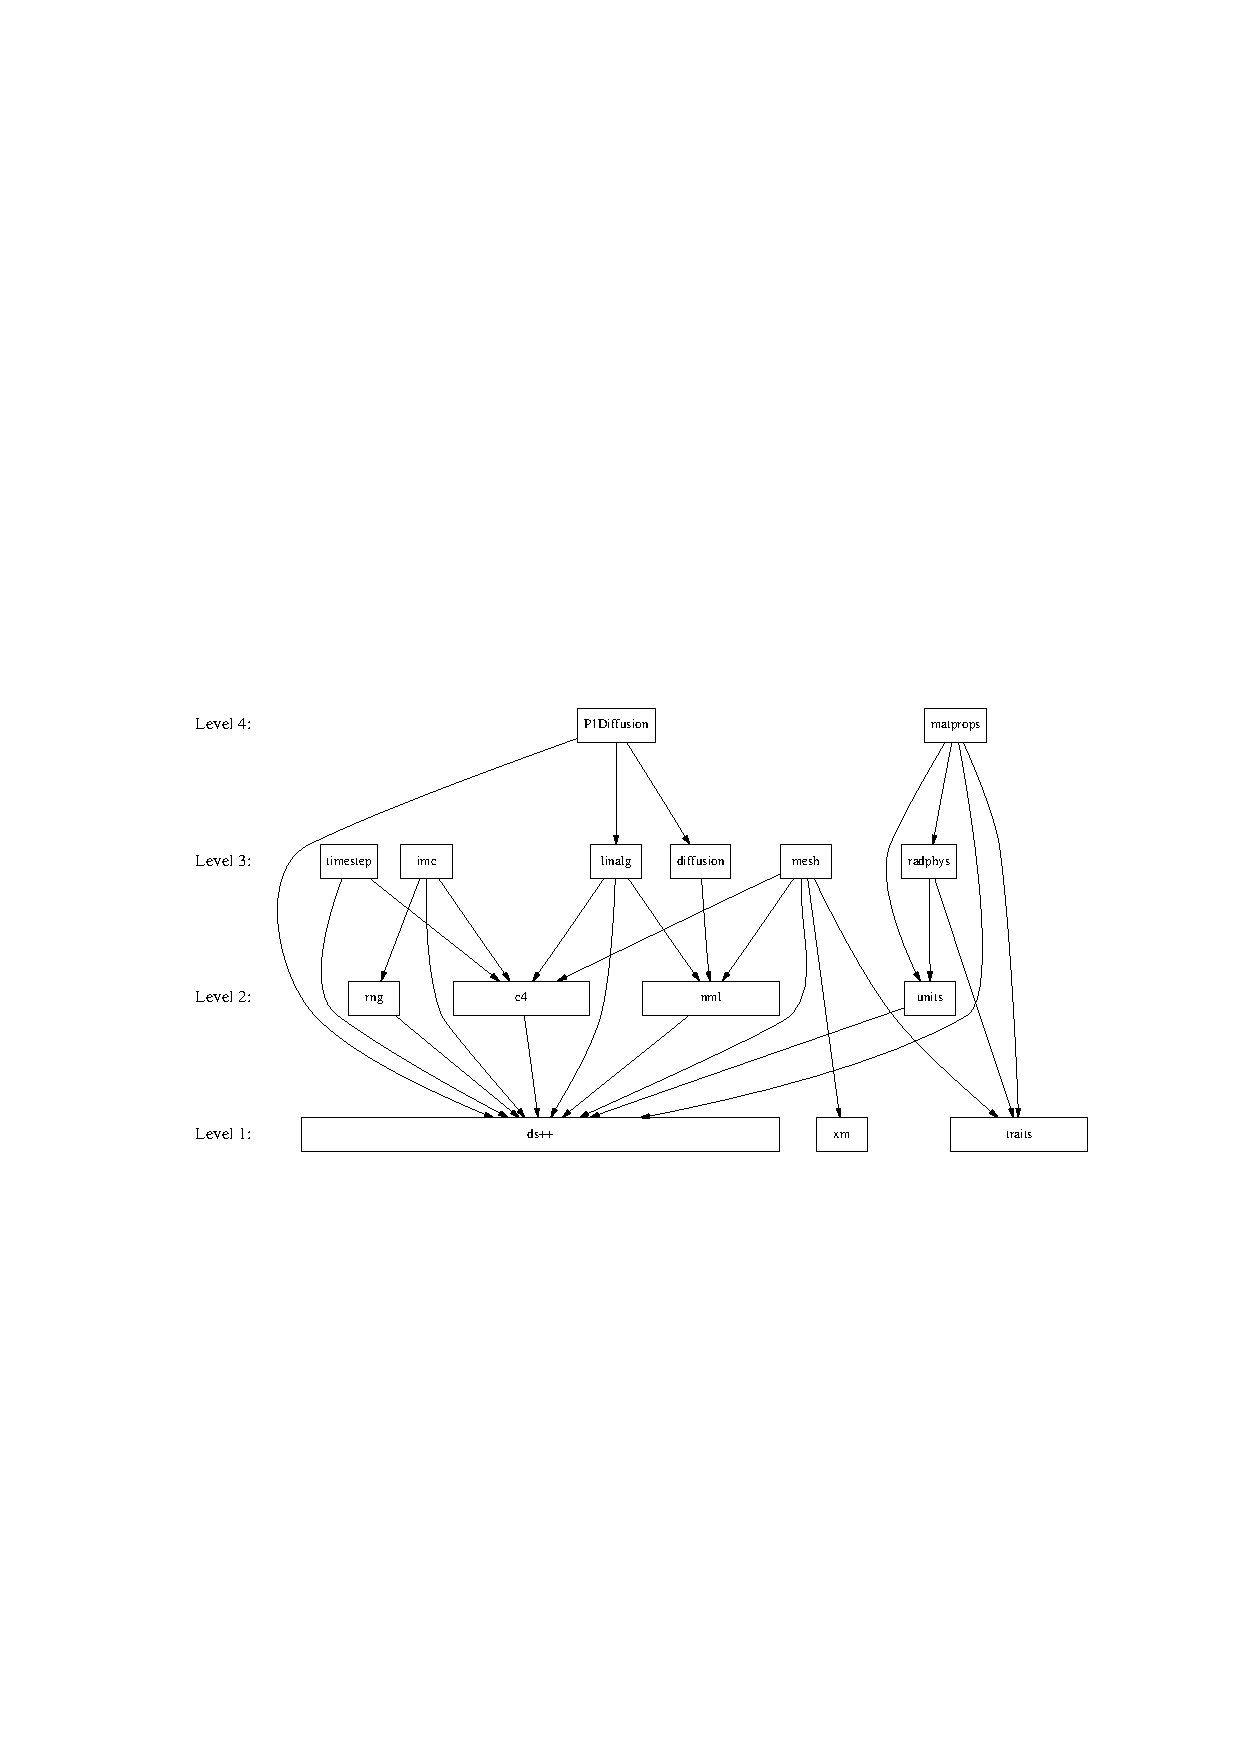
\includegraphics[angle=90]{fig/level}}
  \caption{Component-level diagram for \draco.}
  \label{fig:level}
\end{figure}
of this diagram, one can determine the exact dependencies required by
each component in \draco.  Thus, to compile a component static library, all of
the dependencies, both explicit and implicit, must be included when linking.

In addition to the direct component dependencies illustrated in
Fig.~\ref{fig:level}, the \comp{\vble{pkg}/test/} directory may
require additional components for its compartmentalized unit tests.  For example,
\comp{device} does not explicitly require \comp{c4}, but \comp{c4} and \comp{MPI} are required for compiling the unit tests for \comp{device}.  Unit test dependencies are included in this component-level diagram and dependencies unique to the tests are represented by dotted lines.   
%Figure~\ref{fig:test_level} shows the \draco\ package
%dependency tree
%\begin{figure}
%  \centerline{\includegraphics{fig/test_level.eps}}
%  \caption{Package-level diagram for \draco.  Test dependencies are
%    noted by the dotted arrows.}
%  \label{fig:test_level}
%\end{figure}
%with package test dependencies included.
The policy in \draco\ is that
test directories are responsible for their own template instantiations\index{policy!templates} in \comp{*\_pt.cc} files.
Directions showing how to include test directory dependencies are given in Chap~\ref{chap:adding}. 

When using \draco\ on an external product, all component dependent
libraries must be included.\index{dependencies!component}  The list of necessary libraries for
linking a package is given in Table~\ref{tab:depends}.  In summary,
\begin{table}
  \caption{
    Listing of \draco\ component dependencies.  The \draco\ component
    dependencies are the sum of the explicit and implicit dependencies.
    For general package use, only components listed under \draco\ Component
    Dependencies (Explicit and Implicit) are required.  The components
    listed under \draco\ Component Test Dependencies are only required for
    testing.}
  \label{tab:depends}
  \begin{center}
    \begin{tabular}{lclll} \hline\hline
      \multicolumn{1}{c}{\draco\ Package} & Level &
      \multicolumn{1}{c}{\draco\ Explicit} &
      \multicolumn{1}{c}{\draco\ Implicit} &
      \multicolumn{1}{c}{\draco\ Package} \\ 
      & & \multicolumn{1}{c}{Package Dependencies} &
      \multicolumn{1}{c}{Package Dependencies} &
      \multicolumn{1}{c}{Test Dependencies} \\ \hline
       \dsxx & 1 & - & - & - \\

%       \xm & 1 & - & - & - \\
%       \pkg{nml} & 2 & \dsxx & - & - \\
       \cfour & 2 & \dsxx & - & - \\
       \pkg{cdi} & 2 & \dsxx & - & - \\
       \pkg{fpe\_trap} & 2 & \dsxx & - & - \\
       \pkg{lapack\_wrap} & 2 & \dsxx & - & - \\
       \pkg{linear} & 2 & \dsxx & - & - \\
       \pkg{mesh\_element} & 2 & \dsxx & - & - \\
       \pkg{ode} & 2 & \dsxx & - & - \\
       \pkg{plot2D} & 2 & \dsxx & - & - \\
       \rng & 2 & \dsxx & - & - \\  
       \pkg{shared\_lib} & 2 & \dsxx & - & - \\
       \pkg{traits} & 2 & \dsxx & - & -  \\ 
       \pkg{units} & 2 & \dsxx & - & - \\       
       
%       \pkg{diffusion} & 3 & \pkg{nml} & \dsxx & \pkg{mesh} \\
%         \imc & 3 & \dsxx, \rng, \cfour & - & - \\
%       \pkg{linalg} & 3 & \dsxx, \cfour, \pkg{nml} & - & - \\
%       \pkg{mesh} & 3 & \dsxx, \pkg{xm}, \pkg{traits}, \cfour,
%       \pkg{nml} & - & - \\
%       \pkg{radphys} & 3 & \pkg{traits}, \pkg{units} & - &
%       \pkg{mesh} \\ 
       \pkg{cdi\_ipcress} & 3 & \pkg{cdi} & \dsxx & - \\
       \pkg{cdi\_eospac} & 3 & \pkg{cdi} & \dsxx & - \\
       \pkg{device} & 3 & \dsxx & - & \cfour \\
       \pkg{diagnostics} & 3 & \cfour & \dsxx & - \\
       \pkg{fit} & 3 & \pkg{linear} & \dsxx & - \\
       \pkg{meshReaders} & 3 & \pkg{mesh\_element} & \dsxx & - \\
       \pkg{min} & 3 & \pkg{linear} & \dsxx & - \\
       \pkg{norms} & 3 & \cfour & \dsxx & - \\
       \pkg{parser} & 3 & \cfour, \pkg{units} & \dsxx & - \\
       \pkg{roots} & 3 & \pkg{linear} & \dsxx & - \\
       \pkg{special\_functions} & 3 & \pkg{ode}, \pkg{units} & \dsxx & - \\
       \pkg{timestep} & 3 & \cfour & \dsxx & - \\
       \pkg{viz} & 3 & \pkg{traits} & \dsxx & - \\
       
       \pkg{cdi\_analytic} & 4 & \pkg{parser}, \pkg{ode}, \pkg{cdi} & \cfour, \dsxx, \pkg{units} & - \\
       \pkg{quadrature} & 4 & \pkg{parser},  & \cfour, \dsxx, \pkg{units},  & - \\
        &  & \pkg{mesh\_element},  & \pkg{ode} &  \\
        &  & \pkg{special\_functions} &  &  \\
              
%       \pkg{matprops} & 4 & \dsxx, \pkg{traits}, \pkg{units},
%       \pkg{radphys} & - & \pkg{mesh} \\
%       \pone & 4 & \dsxx, \pkg{linalg}, \pkg{diffusion} & \cfour,
%       \pkg{nml} & \pkg{mesh} \\ 
\hline\hline
    \end{tabular}
  \end{center}
\end{table}
when a \draco\ component is used in an external code, all libraries
listed under \draco\ Package Dependencies (Explicit and Implicit) in
Table~\ref{tab:depends} must be included on the link line.  The
packages listed under \draco\ Package Test Dependencies do not have to
be linked.  We note that \draco\ packages know both their package
dependencies and their package test
dependencies (Fig.~\ref{fig:level}).  The external \draco\ client
must be aware that when using a \draco\ package all of the packages
dependencies (not package test dependencies) must be included.

Some components in \draco\ require external vendor support.\index{dependencies!vendor}
Additionally, some configuration options in \draco\ require external
vendor support.  Table~\ref{tab:vendor} lists all of the present
\begin{table}
  \caption{Vendors required by packages in \draco.  Implicit are the
    \cpp\ Standard Template Library (STL), the \cc\ Standard
    Library, and compiler libraries (\comp{libF77}).  Systems
    libraries  (\comp{sys/time.h}) are also not included.}
  \label{tab:vendor}
  \begin{center}
    \begin{tabular}{lclc}\hline\hline
      \multicolumn{1}{c}{Package} & Level & \multicolumn{1}{c}{Vendor Options}
      & Required \\ \hline
      \dsxx & 1 & - &  - \\
      
%      \xm & 1 & - & - \\
      \cfour & 2 & \mpi, \sys{OpenMP} & no \\
      & & \sys{PAPI} & no \\
      \pkg{cdi} & 2 & - & - \\
      \pkg{fpe\_trap} & 2 & \mpi & no \\
      \pkg{lapack\_wrap} & 2 & \sys{LAPACK}, \sys{BLAS} & yes \\
      \pkg{linear} & 2 & - & - \\
      \pkg{mesh\_element} & 2 & - & - \\
      \pkg{ode} & 2 & - & - \\
      \pkg{plot2D} & 2 & \sys{XM Grace} & yes \\
      \pkg{rng} & 2 & \sys{GSL} & yes \\
      \pkg{shared\_lib} & 2 & \sys{dlopen} & yes \\
      \pkg{traits} & 2 & - & - \\
      \pkg{units} & 2 & - & - \\
      
%      \pkg{nml} & 2 & - & - \\
%      \rng & 2 & \sprng & yes  \\
%      \pkg{units} & 2 & - & - \\
%      \pkg{diffusion} & 3 & - & - \\
%      \imc & 3 & - & -  \\
%      \pkg{linalg} & 3 & \pcglib & yes \\
%      \pkg{mesh} & 3 & - & - \\
    %  \pkg{radphys} & 3 & - & - \\ 
          \pkg{cdi\_eospac} & 3 & \sys{EOSPAC} & yes \\
      \pkg{cdi\_ipcress} & 3 & - & - \\
      \pkg{device} & 3 & \sys{DaCS} or \sys{CUDA} & yes \\
       &  & \sys{MPI} & no \\
      \pkg{diagnostics} & 3 & \sys{MPI} & no \\
      \pkg{fit} & 3 & - & - \\
      \pkg{meshReaders} & 3 & - & - \\
      \pkg{min} & 3 & - & - \\
      \pkg{norms} & 3 & \sys{MPI} & no \\
      \pkg{parser} & 3 & \sys{MPI} & no \\
      \pkg{roots} & 3 & - & - \\
      \pkg{special\_functions} & 3 & \sys{GSL} & yes \\      
      \pkg{timestep} & 3 & \sys{MPI} & no \\
      \pkg{viz} & 3 & - & - \\
       
%      \pkg{matprops} & 4 & - & - \\
%      \pone & 4 & - & - \\ 
      \pkg{cdi\_analytic} & 4 & \sys{MPI} & no \\
      \pkg{quadrature} & 4 & \sys{GSL} & yes \\
       &  & \sys{MPI} & no \\
      \pkg{RTT\_Format\_Reader} & 4 & - & - \\

\hline\hline
    \end{tabular}
  \end{center}
\end{table}
components in \draco\ and the vendors that are required to build those
components.  Also, because \draco\ is based on the concepts of levelized
design as stated above, each component in \draco\ may have dependencies
on lower level \draco\ components.  In these cases only the dependencies
of the specified package are of interest.  For example, the \pkg{parser} 
component itself requires no external vendors; however, \pkg{parser} requires
\cfour\ that does require an external vendors (\sys{MPI}).  The build system
knows the \draco\ dependencies of each component; however, the external
user (client) must be aware of vendor requirements in the component
dependencies.  If a required vendor library is not found by the \draco\ build system, that component will be omitted from the configuration.  For example, if \sys{LAPACK} is not found on the current machine, the \draco\ build system will not attempt to configure or compile \pkg{lapack\_wrap}.  Some dependencies, like \sys{PAPI} are only used for profiling and if activated anywhere, must be activated everywhere.
Tables~\ref{tab:depends} and \ref{tab:vendor} can be
used to determine what \draco\ components and what vendor libraries must
be included when linking to a specific \draco\ components.  Details on
how to configure components with certain vendor options are given in
\S~\ref{sec:configuration_options}.  Information on linking to
specific libraries is given in Appendix~\ref{app:vendor_libs}.

To summarize the preceding we will employ a simple example.  Let us
assume that a user wishes to use the \pkg{quadrature} package.  Additionally,
this configuration will be a parallel configuration using
\mpi\,\footnote{\cfour\ is \draco's communication package and
  determines if the resulting code will be scalar or parallel.}.  From
Table~\ref{tab:depends} we see that \pkg{quadrature} is dependent on the \draco\ 
packages \pkg{special\_functions}, \pkg{parser}, \pkg{mesh\_element}, \pkg{ode}, \dsxx, \pkg{units}, and \cfour.  From Table~\ref{tab:vendor} we see
that \pkg{ode} requires the \sys{GSL} library and \cfour\ requires the \mpi\ 
library.  Accordingly, for a \sys{UNIX} \sys{Makefile}-based build, the following libraries must be included on the
link line:
\begin{verbatim}
     -lrtt_quadrature -lrtt_parser -lrtt_special_functions -lrtt_c4 -lrtt_units \
     -lrtt_mesh_element -lrtt_ode -lrtt_ds++ \
     -lgsl -lgslcblas \
     -lmpi_cxx -lmpi -lopen-rte -lopen-pal
\end{verbatim}
where \comp{-lgsl -lgslcblas} are the \pkg{GSL} libraries (see \S~\ref{appsec:gsl}) and \comp{-lmpi\_cxx -lmpi -lopen-rte -lopen-pal} are the \mpi\ libraries (see \S~\ref{appsec:mpi}).  Additional system libraries may also be required (e.g.: \comp{-ldl -lnsl -lutil -lm}).
This example assumes that all of the following library locations are
defined in \ldlib.  Thus, even though \pkg{quadrature} does not explicitly depend
on \mpi\ or \sys{GSL}, it uses \draco\ packages (\cfour\ and \pkg{special\_functions}) that
do require these libraries.  In practice, the \draco\ build system attempts to find and use full paths to vendor and \draco\ component libraries so that \ldlib\ does not need to be manipulated by the developer or software user.  The build system also locates and sets all of the libraries required or each vendor so that a \draco\ component or client only needs to specify that it should link to a set of libraries provided by the \cmake\ variable  \$\vble{\{\$\{VENDOR\}}\comp{\_LIBRARIES\}}.

%%---------------------------------------------------------------------------%%

\section{Draco Package Products}

In Chap.~\ref{chap:model} we insinuated that each \draco\ component
provides a library.  For example, \pkg{quadrature} provides
\comp{librtt\_quadrature.a(.so)} on \sys{UNIX} systems.  This is not entirely accurate.  Some \draco\
packages, \pkg{traits} is an example, consist only of header files and do not
provide a compiled library.  Users need to be aware of this fact when
linking \draco\ components.  If a \draco\ client uses the \pkg{viz}
package, which requires \pkg{traits}, linking \comp{-lrtt\_traits} is incorrect because
\pkg{traits} does not produce a library.  Table~\ref{tab:products} lists the
\begin{table}
  \caption{Products for \draco\ packages.}
  \label{tab:products}
  \begin{center}
    \begin{tabular}{lccc}\hline\hline
      \multicolumn{1}{c}{Package} & \comp{include/} & \comp{lib/} &
      \comp{bin/} \\ \hline
      
      \dsxx & yes & yes &  no \\
      
      \cfour & yes & yes & no \\
      \pkg{cdi} & yes & yes & no \\
      \pkg{fpe\_trap} & yes & yes & no \\
      \pkg{lapack\_wrap} & yes & no & no \\
      \pkg{linear} & yes & yes & no \\
      \pkg{mesh\_element} & yes & yes & no \\
      \pkg{ode} & yes & yes & no \\
      \pkg{plot2D} & yes & yes & no \\
      \pkg{rng} & yes & yes & no \\
      \pkg{shared\_lib} & yes & yes & no \\
      \pkg{traits} & yes & no & no \\
      \pkg{units} & yes & yes & no \\
      
      
      
      \pkg{cdi\_eospac} & yes & yes & no \\
      \pkg{cdi\_ipcress} & yes & yes & yes \\
      \pkg{device} & yes & yes & no \\
      \pkg{diagnostics} & yes & yes & no \\
      \pkg{fit} & yes & yes & no \\
      \pkg{meshReaders} & yes & yes & no \\
      \pkg{min} & yes & yes & no \\
      \pkg{norms} & yes & yes & no \\
      \pkg{parser} & yes & yes & no \\
      \pkg{roots} & yes & yes & no \\
      \pkg{special\_functions} & yes & yes & no \\
      \pkg{timestep} & yes & yes & no \\
      \pkg{viz} & yes & yes & no \\
                 
      \pkg{cdi\_analytic} & yes & yes & no \\
      \pkg{quadrature} & yes & yes & no \\
      \pkg{RTT\_Format\_Reader} & yes & yes & no \\
      
      \hline\hline
%      \multicolumn{4}{l}{$^{\text a}$\pkg{nml} uses a \perl\ script
%        \comp{nmlgen*} that} \\
%      \multicolumn{4}{l}{is installed in the \comp{libexec/}
%        directory.} \\
    \end{tabular}    
  \end{center}
\end{table}
\draco\ packages and their products.  Users must only link against
those products that make a library.  Note also that package executables
produced under the \vble{pkg}\comp{/test/} directories are not
considered executable products.

%%---------------------------------------------------------------------------%%

\section{Configuring Draco}
\label{sec:configuring_draco}

We have previously mentioned that building \draco\ is a two-step
process.  First, \draco\ must be configured for a particular build configuration and build tool.\index{configuring}
Second, \draco\ is built using particular build targets.  In this
section we shall concentrate on configuring \draco.  Note that many
details about \cmake\ and the \draco\ \cmake\ macros are glossed over in this
treatment.  Interested readers are referred to Ref.~\cite{cmake}
for more information.  Examples that illustrate the concepts described 
in this section are given in \S~\ref{sec:examples}.

\subsection{Preparing the target and binary directories}
\label{sec:running_configure_prepare}

Running \cmake\ is straightforward; however, setting up the target
directories where various builds will take place require some
consideration.  In \S~\ref{sec:draco_src_tree} we described how the
source tree is not necessarily where the build takes place.  In fact,
we advise that builds be performed in a location separate from the
source tree\footnote{The exception to this advice is when the target build tool is \sys{Eclipse CDT} where there are advantages to using a {\it within-source-tree build}, namely, better support for \svn\ through the \sys{Eclipse} IDE.}.  Through this method multiple builds (debug, optimized) can be performed
simultaneously using the same source files.  Additionally, the source tree will not be cluttered
by build-file remnants such as object dependency files.\index{build!within-source-tree}\index{build!out-of-source-tree}

Before running \cmake\ to configure your build directory, we set up target and binary directory trees\index{directory!binary}\index{directory!target}.  Note
that this directory can be the same as the source directory; although,
we do not recommend this strategy.  The target directory name should
be descriptive of the particular build that is being performed.  For
example to build a debug version on a Linux platform with \mpi\ support, one might make
a directory entitled \comp{linux\_\,mpid/}. Thus, for \sys{Unix} systems the user enters
\begin{verbatim}
     $ mkdir -p linux_mpid/draco
\end{verbatim} % $
Similar directory creation processes should be used on other platforms.  Note that we do not require a \comp{draco/} binary directory under the target
directory.  However, this strategy does alleviate the complexity when
using \draco\ with other code systems.  If the user is planning on
using a product that emulates the \draco\ build system, such as
\capsaicin, \clubimc\  or \milagro, then parallel binary directories should be
added for each product
\begin{verbatim}
     $ cd linux_mpid
     $ mkdir capsaicin
     $ mkdir clubimc
     $ mkdir milagro
\end{verbatim}
Details on using the \draco\ build model in external products are
reserved until Chap.~\ref{chap:extern}.

\subsection{Running CMake from the command line}
\label{sec:running_configure_cmd_line}

The next step is to run the \cmake\ command line tool inside the \draco\ binary directory.  If you prefer, you can run the interactive \cmake\ tools described in \S~\ref{sec:running_configure_ccmake} and \S~\ref{sec:running_configure_cmakegui}.  We assume that the \draco\ source tree lives at \dracohome.  
To generate a build project in the binary dreictory, run \cmake\ from the \draco\ binary directory, \comp{linux\_\,mpid/draco/} and provide the location of the \draco\ source tree as a \cmake\ argument.  Most importantly, we need to set the
install directory\index{directory!install}, denoted by \comp{CMAKE\_INSTALL\_PREFIX} on the \cmake\ command line\footnote{This can also be set in the file \comp{linux\_\,mpid/draco/CMakeCache.txt}, or in the GUI interface provided by \comp{ccmake} or \comp{cmake-gui}.}.  To set a build parameter on the \cmake\ command line we use the \cmake\ option \comp{-D}.  An example \cmake\ configuration command for a \sys{UNIX} \sys{Makefile} configuration is illustrated here:
\begin{verbatim}
      $ cd linux_mpid/draco
      $ cmake -DCMAKE_INSTALL_PREFIX=.. $draco_home
\end{verbatim}
The first option sets the install location to the target directory, \comp{linux\_\,mpid/}.  The second option provides the source location of \draco\ and the controlling \comp{CMakeLists.txt} file.
%This may be accomplished in two ways.  One, the
%user may run the \dracoconf\ script that comes with the \draco\ 
%distribution.  This script requires the user to set the
%\comp{--prefix} directory as an argument to the script. The following
%examples illustrate this option:
%\begin{verbatim}
%     $ cd sgi_mpi/draco
%     $ $draco_home/draco_config ..
%     $ $draco_home/draco_config .
%     $ $draco_home/draco_config /usr/local/contrib/draco
%\end{verbatim} % $
%The first option sets the install location in \comp{sgi\_\,mpi/}.  The
%second option sets the install location in \comp{sgi\_\,mpi/draco/}.
%The final option installs in \comp{/usr/local/contrib/draco/}.  The
%\dracoconf\ script will give an error if a \comp{--prefix} directory
%is not given.  
Note that additional options for \cmake\ are simply
appended to the command-line ahead of the source location.  Thus, to force the creation of static libraries for the \draco\ build,
we would enter
\begin{verbatim}
     $ cmake  -DCMAKE_INSTALL_PREFIX=.. -DDRACO_LIBRARY_TYPE=STATIC $draco_home
\end{verbatim}
More details on the configuration options are given in
\S~\ref{sec:configuration_options}.

%The second way to run configure is to manually run the
%\dracohome\comp{/configure*} script.  Thus, to repeat the options from 
%the preceding paragraph, the user must enter
%\begin{verbatim}
%     $ cd sgi_mpi/draco
%     $ $draco_home/configure --prefix=$home/sgi_mpi
%     $ $draco_home/configure --prefix=$home/sgi_mpi/draco
%     $ $draco_home/configure --prefix=/usr/local/contrib/draco
%\end{verbatim} % $
%where we have assumed that \comp{sgi\_\,mpi/} lives in \comp{\$home}.
%The differences between running \dracoconf\ and
%\dracohome\comp{/configure*} should now be apparent.  Configure
%expects the directory specified by \comp{--prefix} to be an absolute
%path.  \dracoconf\ allows the user to enter relative paths, and it
%converts these to absolute paths for configure.  Proceeding with our
%analysis, if the user wants to install \draco\ products in
%\comp{\$home/sgi\_\,mpi/} with \mpi\ then the following is required
%\begin{verbatim}
%     $ $draco_home/configure --prefix=$home/sgi_mpi --with-c4=mpi
%\end{verbatim} % $
%Additional configuration options are detailed in
%\S~\ref{sec:configuration_options}. 

Running \cmake\ in the \comp{draco/} binary directory within the target
directory (\comp{linux\_\,mpid/}) produces a directory tree under
the \comp{draco/} subdirectory that is parallel to the \draco\ source
directory tree.  This directory structure is illustrated in
Fig.~\ref{fig:build_tree}.  Note that we could have run \cmake\ 
under the target top-level directory (\comp{linux\_\,mpid/}).  If we had
proceeded with this strategy the contents of the \comp{draco/} target
subdirectory would be moved up one level.

One final point should be mentioned about \comp{CMAKE\_INSTALL\_PREFIX}.  \cmake's
default location for the installation directory is
\comp{/usr/local/} on \sys{UNIX} and \comp{\%ProgramFiles\%} on \sys{Windows}, but the build system will modify this value to point to an \comp{install} subdirectory located beneath the \draco\ binary diretory (e.g.: \comp{linux\_\,mpid/draco/install}) if the developer does not provide another location.  Thus, the user must enter a value for \comp{CMAKE\_INSTALL\_PREFIX} either on the command line or via the \cmake\ GUI 
explicitly to override the default.  The suggested method is to set
\comp{CMAKE\_INSTALL\_PREFIX} to the target directory (\comp{linux\_\,mpid/} in this
example).  This will allow multiple targets to be built simultaneously 
without risk of name collisions.

If the build configuration requires many options, the developer may choose to create a \comp{CMakeCache.txt} file\index{CMakeCache.txt} in the \draco\ binary directory before running \cmake\ for the first time.  All build options can set in the \comp{CMakeCache.txt} file so that the configuration command only requires the location of the sources:
\begin{verbatim}
    $ cd linux_mpid/draco
    $ ls
    CMakeCache.txt
    $ cmake $draco_home
\end{verbatim}
A sample \comp{CMakeCache.txt} file is provided in the root \draco\ source directory.  The contents of this file are also provided in Listing~\ref{lst:cmakecachetxt}.
%
\lstset{language=ksh,
  showstringspaces=false,
  frame=shadowbox,
  basicstyle=\footnotesize,
  rulesepcolor=\color{black},
  backgroundcolor=\color{listingBG}
}
\begin{lstlisting}[basicstyle=\footnotesize, xleftmargin=0.0in, xrightmargin=0.0in, caption={A sample \comp{CMakeCache.txt} file.}, float=tn,label={lst:cmakecachetxt}]
# CMakeCache.txt template for Draco
# $Id$

# Instructions.
# 1. Copy this file to your build directory as CMakeCache.txt.
# 2. Review and update all values in this file.
# 3. From the build directory run 'cmake /full/path/to/source'
# 4. make
# 5. ctest
# 6. make install

# ------------------------------------------------------------
# You must set these values for your build:
# ------------------------------------------------------------

# Location where 'make install' will copy files to.
# CMAKE_INSTALL_PREFIX:PATH=c:/Release-x64/draco
CMAKE_INSTALL_PREFIX:PATH=/var/tmp/kgt/cmake/gcc/mpid/t

# VENDOR_DIR:PATH=$ENV{VENDOR_DIR}
# Windows: k:/vendors/x64-Windows
VENDOR_DIR:PATH=/ccs/codes/radtran/vendors/Linux64

# CMAKE_BUILD_TYPE == { Release, Debug, RelWithDebInfo, MinSizeRel }
CMAKE_BUILD_TYPE:STRING=Debug

# CMAKE_GENERATOR == { NMake Makefiles, Unix Makefiles, 
#                      Visual Studio 9 2008, Visual Studio 9 2008 Win64 }
CMAKE_GENERATOR:STRING=Unix Makefiles

# ------------------------------------------------------------
# Review these additional settings
# ------------------------------------------------------------

# Should we compile the tests?
BUILD_TESTING:BOOL=ON

# C4 communication mode (SCALAR or MPI)
DRACO_C4:STRING=MPI

# Design-by-Contract (0-7)?
DRACO_DBC_LEVEL:STRING=7
 
# Keyword for creating new libraries (STATIC or SHARED).
DRACO_LIBRARY_TYPE:STRING=SHARED
\end{lstlisting} \index{CMakeCache.txt} \index{generator}
Developers can copy this file to the \draco\ binary directory and modify, comment out or add options as needed before running \cmake\ for the first time.

One final note about running \cmake\ from the command line is the option to choose a project {\it Generator}\index{generator}\index{cmake!generator}.  On \sys{UNIX} systems, the default generator is \sys{Unix Makefiles}, but \sys{Eclipse CDT4 - Unix Makefiles} is also supported.  To select an alternative generator, use the \comp{-G} command line argument for \cmake.  The full list of available generators can be obtained by running \comp{'cmake --help'}.

%% ---------------------------------------------------------------------------- %%
\subsection{Running CMake interactively from the command line}
\label{sec:running_configure_ccmake}

\cmake\ can be run in an interactive environment by running \comp{ccmake} from command line\index{ccmake}.  This configuration mode is similar to the the method described above in \S~\ref{sec:running_configure_cmd_line}.  To start the interactive configure session, navigate to the binary directory and run \comp{ccmake}
\begin{verbatim}
     $ cd linux_mpid/draco
     $ ccmake $draco_home
\end{verbatim}
This will start an interactive configure session that will look similar the screenshot shown in Listing~\ref{lst:ccmake-empty}.
\begin{lstlisting}[basicstyle=\footnotesize, xleftmargin=0.0in, xrightmargin=0.0in, caption={The \comp{ccmake} screen prior to running configure.}, float=htn, label={lst:ccmake-empty}]
                                                     Page 0 of 1
 EMPTY CACHE


EMPTY CACHE:                                                                              
Press [enter] to edit option                                       CMake Version 2.8.8-rc1
Press [c] to configure
Press [h] for help           Press [q] to quit without generating
Press [t] to toggle advanced mode (Currently Off)
\end{lstlisting}
Selecting interactive command \comp{[c]} (followed by \comp{[e]} to exit the output review screen) 
will populate the configure environment with default values (be sure to turn caps lock off) resulting in something similar to what is shown in Listing~\ref{lst:ccmake-post-configure}.
\begin{lstlisting}[basicstyle=\footnotesize, xleftmargin=0.0in, xrightmargin=0.0in, caption={The \comp{ccmake} screen after the initial configure command.}, float=htn, label={lst:ccmake-post-configure}]
                                                     Page 1 of 1
 BUILD_AUTODOC                   *OFF                                                    
 BUILD_DOC                       *OFF                                                    
 BUILD_TESTING                   *ON                                                     
 BUILD_USE_SOLUTION_FOLDERS      *ON                                                     
 CMAKE_BUILD_TYPE                *Debug                                                  
 CMAKE_INSTALL_PREFIX            */var/tmp/gcc-mpid/d/install                        
 DRACO_C4                        *MPI                                                    
 DRACO_DBC_LEVEL                 *7                                                      
 DRACO_DIAGNOSTICS               *0                                                      
 DRACO_LIBRARY_TYPE              *SHARED                                                 
 DRACO_TIMING                    *0                                                      
 DRACO_VERSION                   *6.3                                                    
 DRACO_VERSION_FULL              *6.3.20120412                                           
 ENABLE_RNG_NR                   *OFF                                                    
 GCC_ENABLE_ALL_WARNINGS         *OFF                                                    
 GCC_ENABLE_GLIBCXX_DEBUG        *OFF                                                    
 GSL_FOUND                       *ON                                                     
 NUMDIFF                         */ccs/codes/radtran/vendors/numdiff-5.2.1/bin/numdiff   
 USE_OPENMP                      *ON                                                     
 VENDOR_DIR                      *              

BUILD_AUTODOC: OFF                                                                                                                                                         
Press [enter] to edit option                                       CMake Version 2.8.8-rc1
Press [c] to configure
Press [h] for help           Press [q] to quit without generating
Press [t] to toggle advanced mode (Currently Off)
\end{lstlisting}
To modify the target location navigate to the \comp{CMAKE\_INSTALL\_PREFIX} line and press enter to edit the path location.  \comp{ccmake} navigation and editing commands can
be found by selecting the \comp{[h]} option.  Similarly, the build can be configured to generate static libraries by editing the \comp{DRACO\_LIBRARY\_TYPE} value and setting it to \comp{STATIC}.  Once the build settings are complete, select the \comp{[c]} (configure) option two more times to complete the configuration process and review the new values.    To generate the controlling build project files (e.g.: \sys{Makefiles}), select the \comp{[g]} (generate) option.  The most common build features are shown in the default \comp{ccmake} environment.  In some cases, the developer may need to edit an {\it advanced} build variable.  The list of all variables can be viewed by the \comp{[t]} (toggle) advanced values option.

%% ---------------------------------------------------------------------------- %%
\subsection{Running CMake interactively through the GUI}
\label{sec:running_configure_cmakegui}

\cmake\ can be run in an interactive graphical user interface (GUI) by running \comp{cmake-gui} either from the command line for by selecting the tool from the operating system's toolbar (this tool may not be available for all systems).\index{cmake-gui}  This configuration mode is similar to the the methods described above in \S~\ref{sec:running_configure_cmd_line}-\ref{sec:running_configure_ccmake}.  This tool can be started from any directory because the source and binary locations must always be provided manually, when using the GUI tool.  As in the previous section, after providing the source and binary directory locations, select the {\it Configure} button to populate the Cache with default values.  Before the configuration begins, the GUI will request that you select a {\it Generator}.  This discussions assumes that you have selected \sys{Unix Makefiles} as the generator.  After the initial configure, the GUI should appear similar to Fig.~\ref{fig:cmakegui_defaults}.  As in \S~\ref{sec:running_configure_ccmake}, edit the values as needed and rerun the {\it configure} and {\it generate} options to generate the desired build project.
%
\begin{figure}
  \centerline{\includegraphics[angle=0,width=5.5in]{fig/cmakegui_defaults}}
  \caption{CMake GUI after populating cache with default values.}
  \label{fig:cmakegui_defaults}
\end{figure}
%

%% ---------------------------------------------------------------------------- %%
\subsection{Configuration Options}
\label{sec:configuration_options}

Because \draco\ has many packages it must support many configurations.
Additionally, some of these options can be matrixed.  For example,
\draco\ can be configured for 64-bit or 32-bit machines, scalar or parallel, with shared libraries or
archived libaries, and so forth.  The options that one gives during the \cmake\ 
configure step specify most of these options. Also, the build
system has built-in intelligence that will try to make the right
choice if incomplete listings for various options are specified.

For the standard set of \cmake\ options, see Ref.~\cite{cmake}.  The full set of configure options may be examined by running the \cmake\ interactive sessions (\comp{ccmake} or \comp{cmake-gui}).  Some options may only appear on specific systems, after specific vendor installations are discovered, or for specific {\it generators}.  This is the reason that you may need to run {\it configure} more than once when using the interactive versions of \cmake.
%For the standard set of configure options, see Ref.~\cite{autoconf}.
%The full set of configure options may be reproduced at the
%command-line by entering
%\begin{verbatim}
%     $ $draco_home/draco_config --help
%\end{verbatim}
%or 
%\begin{verbatim}
%     $ $draco_home/configure --help
%\end{verbatim}
%Note that from this point onward, we will only give examples using
%\dracoconf. 
As mentioned in the previous section, the built-in configure variable, \comp{CMAKE\_INSTALL\_PREFIX}, should be set explicitly (usually to the target directory) by the
user to avoid installation of \draco\ components in \comp{/usr/local/}.  Alternately, the developer may consider the use of \cmake's \comp{DESTDIR} feature (See \href{http://www.cmake.org/Wiki/CMake_FAQ#Does_CMake.27s_.22make_install.22_support_DESTDIR.3F}{CMake FAQ}).

Configuration options come in four forms: \comp{FILEPATH}, \comp{PATH}, \comp{STRING} and \comp{BOOL}\footnote{There are actually variable types in \cmake.  The 5th type is \comp{INTERNAL}, but this type is not available for user manipulation.}.\index{cmake!variable types}   \draco\ policy is to name \comp{BOOL} options prefixed with \comp{ENABLE\_} or \comp{USE\_}, although there are some exceptions to this policy and this policy is not adopted by \cmake\ built-in variables.  Other variable names should be prefixed with a name to provide context.  This provides a sorted in list the \comp{CMakeCache.txt} file and in the \comp{ccmake} interface and it allows groupings to be collapsed in the GUI.  This policy of using prefix context strings is a \cmake\ and a \draco\ policy standard.
Table~\ref{tab:draco-enable} lists the complete set of \comp{BOOL}
\begin{table}
  \caption{List of \comp{BOOL} options that are unique to \draco.}
  \label{tab:draco-enable}
  \begin{center}
    \begin{tabular}{lcp{3in}} \hline\hline
      \multicolumn{1}{c}{Option} & \multicolumn{1}{c}{Default Value} &
      \multicolumn{1}{c}{Description} \\ \hline
                                % --enable-shmem
%      \comp{--enable-shmem} & off & turns on \shmem\ communication
%      library \\
                                % --enable-pcglib
%      \comp{--enable-pcglib} & on & turns off \pcglib \\
                                % --enable-shared
%      \comp{--enable-shared} & off & turns on shared (\comp{.so})
%      libraries \\
%                                % --enable-static-ld
%      \comp{--enable-static-ld} & off & tries to use static
%      (\comp{.a}) libraries for linking \\
%                                % --enable-strict-ansi
%      \comp{--enable-strict-ansi} & on & compiles using \comp{strict}
%      flags for ANSI compliance \\
%                                % --enable-debug
%      \comp{--enable-debug} & off & turns on \comp{-g} option for
%      debugging$^{\text{a}}$ \\ 
%                                % --enable-32-bit
%      \comp{--enable-32-bit} & off & turns on 32-bit compiling on SGIs 
%      \\
\comp{ENABLE\_RNG\_NR} & OFF & Selects the non-reproducible random number generator feature \\
\comp{USE\_OPENMP} & ON & Disables OpenMP pragmas when compiling \draco\ sources \\
\comp{BUILD\_AUTODOC} & OFF & Enables discovery of Doxygen and the \comp{autodoc} build target \\
%\comp{BUILD_DOC} & OFF & Enables building of all \LaTeX\ documentation found in the \comp{doc} directory \\
\comp{BUILD\_TESTING} & ON & Allows developers to omit configuring for and building code found in test directories (disables \ctest\ features) \\
\comp{BUILD\_USE\_SOLUTION\_FOLDERS} & ON & Only available for \sys{Visual Studio} and \sys{X-Code} generators; makes each \draco\ component a solution folder \\
\comp{CMAKE\_VERBOSE\_MAKEFILE}$^{\text{a}}$ & OFF & Forces the make process to echo all commands to the screen during the build process \\
\comp{GCC\_ENABLE\_ALL\_WARNINGS} & OFF & When using gcc, enable more compiler warning features \\
\comp{GCC\_ENABLE\_GLIBCXX\_DEBUG} & OFF &  When using gcc, use alternate glibc library that provides bounds checking and more safety features \\

              \hline\hline
% footnote
      \multicolumn{3}{p{6in}}{$^{\text{a}}${\footnotesize this option is provided by \cmake\ and is not unique to \draco.  It is provided here because it is a commonly used feature.}}
                                % footnote
%      \multicolumn{3}{l}{$^{\text{a}}$the \KCC\ compiler automatically 
%        includes \comp{-g} support for optimization level \comp{K0},
%        see \S~\ref{sec:optimization}.}
    \end{tabular}
  \end{center}
\end{table}
switches that are unique to \draco.  To turn off a switch the user has
two options, \comp{-DENABLE\_SWITCH=OFF} or run an interactive \cmake\ session and toggle the value.  See Ref.~\cite{cmake} for more details concerning \cmake\ variables.

The \comp{PATH}, \comp{FILEPATH} and \comp{STRING} \cmake\ configure options take actual string arguments.
Table~\ref{tab:draco-with} lists commonly used argument based configure options for \draco.  Some of these are restricted to values provided by a drop down list in the GUI.
\begin{table}
  \caption{List of value based options that are unique to \draco.}
  \label{tab:draco-with}
  \begin{center}
    \begin{tabularx}{\linewidth}{
        >{\setlength{\hsize}{1.0\hsize}}X %
        >{\setlength{\hsize}{.6\hsize}}X %
        >{\setlength{\hsize}{.6\hsize}}X  %
%        >{\setlength{\hsize}{1.1\hsize}}X %
        >{\setlength{\hsize}{1.7\hsize}}X}
      \hline\hline
                                % TABLE HEADINGS
      \multicolumn{1}{c}{Option} & \multicolumn{1}{c}{Valid Arguments} 
      & \multicolumn{1}{c}{Default Value} 
%      & \multicolumn{1}{c}{Implied Argument} 
& \multicolumn{1}{c}{Description} \\ 
\hline\hline
%                                % --with-mpi
%      \comp{--with-mpi} & \comp{vendor mpich} & \comp{no} &
%      \comp{vendor} & see \S~\ref{sec:vendor_libs} \\
%                                % --with-mpi-inc
%      \comp{--with-mpi-inc} & \vble{dir} & \cnull &
%      \comp{\$MPI\_\,INC\_\,DIR} & see \S~\ref{sec:vendor_libs} \\ 
%                                % --with-mpi-lib
%      \comp{--with-mpi-lib} & \vble{dir} & \cnull &
%      \comp{\$MPI\_\,LIB\_\,DIR} & see \S~\ref{sec:vendor_libs} \\
%                                % --with-shmem-inc
%      \comp{--with-shmem-inc} & \vble{dir} & \cnull &
%      \comp{\$SHMEM\_\,INC\_\,DIR} & see \S~\ref{sec:vendor_libs} \\ 
%                                % --with-shmem-lib
%      \comp{--with-shmem-lib} & \vble{dir} & \cnull &
%      \comp{\$SHMEM\_\,LIB\_\,DIR} & see \S~\ref{sec:vendor_libs} \\
%                                % --with-sprng
%      \comp{--with-sprng} & \comp{lfg lcg} & \comp{lfg} & \comp{lfg} &
%      see \S~\ref{sec:vendor_libs} \\
%                                % --with-sprng-inc
%      \comp{--with-sprng-inc} & \vble{dir} & \cnull & 
%      \comp{\$SPRNG\_\,INC\_\,DIR} & see \S~\ref{sec:vendor_libs} \\ 
%                                % --with-sprng-lib
%      \comp{--with-sprng-lib} & \vble{dir} & \cnull &
%      \comp{\$SPRNG\_\,LIB\_\,DIR} & see \S~\ref{sec:vendor_libs} \\
%                                % --with-pcglib-lib
%      \comp{--with-pcglib-lib} & \vble{dir} & \cnull &
%      \comp{\$PCGLIB\_\,LIB\_\,DIR} & see \S~\ref{sec:vendor_libs} \\
%                                % --with-c4
%      \comp{--with-c4} & \comp{scalar mpi shmem} & \comp{scalar} &
%      \comp{scalar} & see \S~\ref{sec:c4_lib} \\
%                                % --with-dbc
%      \comp{--with-dbc} & \comp{0,1,...,7} & \vble{default} &
%      \vble{default} & see \S~\ref{sec:dbc} \\
%                                % --with-opt
%      \comp{--with-opt} & \comp{0,1,2,3} & \comp{0} & \comp{0} & see
%      \S~\ref{sec:optimization} \\
%                                % --with-posix
%      \comp{--with-posix} & \vble{posix src. num.} & \comp{199309L} &
%      \comp{199309L} & sets POSIX source version \\
%                                % --with-mips
%      \comp{--with-mips} & \comp{1,2,3,4} & \comp{mips4} & \comp{4} &
%      sets instruction set on SGIs \\
      	
      \comp{NUMDIFF} & \comp{FILEPATH} to \sys{numdiff} & automatic discovery &  tool used by testing system for comparing output to gold standard output. \\
      \comp{VENDOR\_DIR} & \comp{PATH} & empty & location used by build system for auto discovery of vendor software. \\
      \comp{DRACO\_C4} & MPI or SCALAR & MPI$^{\text{a}}$ & see \S~\ref{sec:vendor_libs} \\
      \comp{DRACO\_DBC\_LEVEL} & 0-7 & 7$^{\text{b}}$ &  see \S~\ref{sec:dbc} \\
      \comp{DRACO\_DIAGNOSTICS} & 0-7 & 0 &  see \S~\ref{sec:diagnostics} \\
      \comp{DRACO\_LIBRARY\_TYPE} & STATIC or SHARED & SHARED &  toggle compilation of archive or shared object (DLL) libraries \\
      \comp{DRACO\_TIMING} & 0-2 & 0 &  see \S~\ref{sec:diagnostics} \\
      \comp{DRACO\_VERSION} & \comp{STRING} & hard coded$^{\text{c}}$ & string that represents the current version of \draco.  This is embedded into the installed \draco\ products. \\
      \comp{DRACO\_VERSION\_FULL} & \comp{STRING} & hard coded$^{\text{c}}$ & string that represents the current version of \draco.  This is embedded into the installed \draco\ products. \\
      
      \hline
      
      \comp{CMAKE\_BUILD\_TYPE} & Debug or Release or RelWithDebInfo or MinSizeRel & Debug & choose type build type; default compiler flags are triggered based on this selection. \\
      \comp{CMAKE\_CXX\_COMPILER} & \comp{FILEPATH} to compiler & \comp{\$ENV{CXX}} & \cpp\ compiler chosen for build.\\
      \comp{CMAKE\_C\_COMPILER} & \comp{FILEPATH} to compiler & \comp{\$ENV{CC}} & C compiler chosen for build. \\
      \comp{CMAKE\_Fortran\_COMPILER} & \comp{FILEPATH} to compiler & \comp{\$ENV{FC}} & Fortran compiler chosen for build. \\
      \comp{CMAKE\_INSTALL\_PREFIX} & \comp{PATH} & \comp{\${BINARY\_DIR} /target} & location for installing \draco (libraries, headers, executables, etc). \\
      
      \hline
      
      {\it VENDOR\_VARIABLE} & varies & automatic discovery & configuration of vendors is done automatically by the \draco\ build system. See \S~\ref{sec:vendor_libs}. \\
      
      \hline\hline
% footnote
      \multicolumn{4}{p{6in}}{$^{\text{a}}${\footnotesize MPI if \sys{MPI} can be found, otherwise SCALAR.}} \\
      \multicolumn{4}{p{6in}}{$^{\text{b}}${\footnotesize The default is 7 for DEBUG builds and 0 for RELEASE (optimized) builds.}} \\
      \multicolumn{4}{p{6in}}{$^{\text{c}}${\footnotesize The version string is built from hard coded values \comp{DRACO\_VERSION\_MAJOR} and \comp{DRACO\_VERSION\_MINOR} hard coded in the top level \comp{CMakeLists.txt}. The patch revision number is set to the configure date for development builds.  Scripts used for releases set the patch version manually.}} 
    \end{tabularx}
  \end{center}
\end{table}
Notice that the build system will automatically populate all fields with default values so that \draco\ can be configured without supplying values for every possible feature.
%\comp{--with} can be used without arguments.  In this case
%an implied argument is assumed by configure.  Thus, \comp{--with}
%options have a default value and an implied argument value.  In the
%first case, a default value is inferred by configure if the
%\comp{--with} option is absent.  In the latter case, an implied
%argument is provided if the \comp{--with} option is present but does
%not specify an argument.
For example, the following two configurations are equivalent because the default value for \comp{DRACO\_C4} is \comp{MPI} if \sys{MPI} can be found on the local system.
\begin{verbatim}
     $ cmake -DDRACO_C4=MPI $draco_home
     $ cmake $draco_home 
\end{verbatim}
In each case, the \cfour\ package is configured for parallel operation with \sys{MPI}.  In the first
case an explicit argument is given.  In the second case  the default value for
\comp{DRACO\_C4} is used.  Not all cases have the same defaults for
options and arguments.  An example is the \comp{MPI\_LIBRARY}
option.  The default is the value returned from the \cmake\ built-in function \comp{find\_package(MPI)}.  For more information about configuring and auto-discovery of vendor software see \S~\ref{sec:vendor_libs} below.
% If the option is given without an argument, configure sets
%\comp{--with-mpi-inc=\$MPI\_\,INC\_\,DIR}. In general, the class of
%\comp{--with} options that load external libraries work in this
%fashion.  Most other \comp{--with} options have the same defaults as
%implied arguments.  On a final note, we do not recommend the practice
%of setting \comp{--without} because \comp{--with} options are not
%meant for binary-type operations.  An exception to this rule is the
%vendor-associated options described in \S~\ref{sec:vendor_libs}.


%% ---------------------------------------------------------------------------- %%
\subsubsection{Vendor Libraries}
\label{sec:vendor_libs}

\draco\ uses external vendors whenever possible to reduce the ammount
of code development required by \draco\ package developers.  The
following vendors are used by \draco:
\begin{itemize}
\item \mpi\ communication library, see \S~\ref{appsec:mpi};
\item \pkg{GSL}, GNU Scientific Library, provides a wide range of mathematical routines such as random number generators, special functions and least-squares fitting, see \S~\ref{appsec:gsl};
\item \pkg{LAPACK} and \pkg{BLAS} provide optimized linear algebra algorithms, see \S~\ref{appsec:lapack};
\item \pkg{CUDA} provides support for running threads on Graphic Processing Units, GPUs, see \S~\ref{appsec:cuda};
\item \pkg{DaCS} provides support for running threads on IBM cell processing units, see \S~\ref{appsec:dacs};
\item \pkg{XMGRACE} provides a 2D plotting capability, see \S~\ref{appsec:grace};
%\item \shmem\ communication library, see \S~\ref{appsec:shmem};
%\item \sprng\ random number library, see \S~\ref{appsec:sprng};
%\item \pcglib\ parallel conjugate gradient solver, see  \S~\ref{appsec:pcglib}.
\end{itemize}\index{vendor!MPI}\index{vendor!GSL}\index{vendor!LAPACK}\index{vendor!CUDA}\index{vendor!Grace}
Vendors are accessed through the \draco\ build system via automatic discovery.  
%using defined \comp{--with} and \comp{--enable} tags in \autoconf.
Table~\ref{tab:vendortags} lists the environment and build system variables that can be manipulated by the developer to alter the discovery process.
\begin{table}
  \caption{Environment and build system variables used to specify vendors in \draco.  See Tables~\ref{tab:draco-enable} and \ref{tab:draco-with} for variable defaults.}
  \label{tab:vendortags}
  \begin{center}
    \begin{tabular}{lap{3.5in}}
    \hline\hline
      \multicolumn{1}{c}{Vendor} & \multicolumn{1}{c}{Variable} & \multicolumn{1}{c}{Details} \\
      \hline
% MPI
      \mpi$^{\text{a}}$ & ENV\{PATH\} & The build system looks for \comp{mpirun} in the current \comp{PATH}. \\
      & MPIEXEC & The full path to the \comp{mpirun} program.  This may need to be set manually if the program has a non standard name like \comp{aprun}. \\
      & MPIEXEC\_NUMPROC\_FLAG & The string used to specify then number of processors to use. Defaults to \comp{'-np'}. \\ 
      & MPI\_C\_LIBRARIES & Manually specify the full paths to \sys{MPI} libraries. \\
      & MPI\_CXX\_LIBRARIES  & \\
      & MPI\_Fortran\_LIBRARIES & \\
      & MPI\_C\_INCLUDE\_PATH & Manually specify the full path to the \sys{MPI} include directory. \\
      & MPI\_CXX\_INCLUDE\_PATH & \\
      & MPI\_Fortran\_INCLUDE\_PATH & \\
      \hline
% LAPACK/BLAS      
      \pkg{LAPACK} & BLA\_STATIC & Look for archive (static) \pkg{LAPACK} and \pkg{BLAS} libraries. Default is ON. \\
      & BLA\_VENDOR & Use a particular type of \pkg{LAPACK} installation like \sys{ATLAS} or \sys{Intel10\_64lp\_gf\_sequential}$^{\text{b}}$. \\
      & ENV\{LD\_LIBRARY\_PATH\} & To help the build system find \pkg{LAPACK}, ensure that the library location is appended to this environment variable. \\ 
      & ENV\{LAPACK\_LIB\_DIR\} & To load a specific \pkg{LAPACK}, ensure this variable is set to the desired location. \\
      \hline
% GSL
      \pkg{GSL} & ENV\{GSL\_INC\_DIR\} & Help the build system find the desired installation by setting this environment variable. \\
      &  ENV\{GSL\_LIB\_DIR\} & Help the build system find the desired installation by setting this environment variable. \\
      \hline
% XMGRACe
      \pkg{XMGrace} & ENV\{GRACE\_INC\_DIR\} & Help the build system find the desired installation by setting this environment variable. \\
      &  ENV\{GRACE\_LIB\_DIR\} & Help the build system find the desired installation by setting this environment variable. \\
      \hline
% CUDA
     \pkg{CUDA}$^{\text{c}}$ &  ENV\{PATH\} & The build system looks for \comp{nvcc} in the current \comp{PATH}. \\
     & CUDA\_NVCC\_FLAGS & Modify the \comp{nvcc} compiler flags. Default is \comp{'-arch=sm\_21'}. \\
     & CUDA\_TOOLKIT\_ROOT\_DIR & If the build system cannot find \comp{nvcc}, the developer must set this location to enable \pkg{CUDA}. \\
     & CUDA\_BIN\_PATH & To use a non-standard location, set this before running \cmake. \\
     
% SHMEM
%      \shmem & --enable-shmem \\
%      & --with-shmem-inc \\
%      & --with-shmem-lib \\ \hline
% SPRNG
%      \sprng & --with-sprng \\
%      & --with-sprng-inc \\
%      & --with-sprng-lib \\ \hline
% PCGLIB
%      \pcglib & --enable-pcglib \\
%      & --with-pcglib-lib \\
      \hline\hline
      % footnotes
      \multicolumn{3}{p{6in}}{$^{\text{a}}${\footnotesize Run \comp{'cmake --help-module FindMPI'} for more details on the discovery process for \pkg{MPI}.}} \\
      \multicolumn{3}{p{6in}}{$^{\text{b}}${\footnotesize To obtain a list of support installations of \pkg{LAPACK}, see the documentation for \cmake's \comp{FindLAPACK.cmake} module (try \comp{'cmake --help-module FindLAPACK'}).}} \\
      \multicolumn{3}{p{6in}}{$^{\text{c}}${\footnotesize Run \comp{'cmake --help-module FindCUDA'} for more details on the discovery process for \pkg{CUDA}.}} \\
    \end{tabular}
  \end{center}
\end{table}
Tables~\ref{tab:draco-enable} and \ref{tab:draco-with} list additional controls that can manipulate how each vendor is used in \draco.  Details on how to use
these variables are given below.

\draco\ vendor libraries are of two types; \latin{required} and
\latin{optional}.  The type classification for each vendor is found in
Table~\ref{tab:vendor}.  \draco\ treats vendors according to the
following rules:
\begin{enumerate}
\item Required vendor libraries are on by default and the configuration will {\bf fail} if the libraries cannot be located;
\item Optional vendor libraries are on by default but the configuration will {\bf pass} if the libraries cannot be located.
\end{enumerate}
For example, \pkg{GSL} is a required vendor.  If \pkg{GSL} cannot be found, the project will not be configured and  cannot be built.  If the optional vendor \pkg{XMGrace} cannot be found, the configuration will be successful, but the \draco\ component \pkg{plot2D} will be omitted because it requires \pkg{XMGrace}.  Finally, if the optional vendor \pkg{MPI} cannot be found the configuration will be sucessful, but the \cfour\ component will be built with the \comp{SCALAR} option instead of \comp{MPI}.  Review Table~\ref{tab:depends} to determine what components may be omitted when vendor libraries are not found. This concept applies to all vendor libraries.

%We note that these rules are applied on a package-by-package basis.
%For example, \sprng\ is only required for \rng; thus, \sprng\ is on in
%the \rng\ and \imc\ packages (see Table~\ref{tab:depends}).  It is
%undefined everywhere else.  

%As illustrated in Table~\ref{tab:vendortags}, vendor options are set
%by the following three configure tags:
%\begin{enumerate}
%\item \comp{--with-\vble{vendor}} (\comp{--enable-\vble{vendor}})
%  turns the vendor on or off.  If the vendor has options (e.g.
%  \comp{--with-mpi}) then \comp{--with} is used.  If the vendor is
%  simply on or off (e.g.  \comp{--enable-shmem}) then \comp{--enable}
%  is used.
%\item \comp{--with-\vble{vendor}-inc} overrides the default \soft{cpp}
%  search locations for header files if the vendor is on.
%\item \comp{--with-\vble{vendor}-lib} overrides the default search
%  path (\ldlib) for libraries if the vendor is on.
%\end{enumerate}
%Optional vendors may be turned on simply by setting
%\comp{--with-\vble{vendor}-inc} or \comp{--with-\vble{vendor}-lib}.
%If these tags are set without setting \comp{--with-\vble{vendor}} then
%the optional library is turned on, and \comp{--with-\vble{vendor}}
%takes the value of its implied argument.  Libraries that use a
%\comp{--enable} tag are simply on in this case.  Naturally, the
%headers and libraries are searched in the directories given by
%\comp{--with-\vble{vendor}-inc} and \comp{--with-\vble{vendor}-lib}.
%For required vendors, setting \comp{--with-\vble{vendor}-inc} or
%\comp{--with-\vble{vendor}-lib} simply changes the default search
%locations for headers and libraries as explained above.

% We note that if an optional vendor is not found by the build system then
% the packages that depend on these vendors will not build.  
%%In other
%%words, required vendors need not be turned off even if the packages
%%that use them are not part of a specific \draco\ distribution.
% \draco\ knows what packages require what vendors, so optional vendor libraries that are missing
% in a particular distribution will have no effect on the rest of the packages.

%% ---------------------------------------------------------------------------- %%
\subsubsection{C4 Package Options}
\label{sec:c4_lib}

\cfour\ is \draco's parallel communication package.  It uses \mpi\ 
%either \mpi\ or \shmem\ 
to perform message passing operations.  Therefore, \cfour\ is intimately connected to the \mpi\ 
%and \shmem\ 
vendor.  The \cmake\ variable \comp{DRACO\_C4} determines how \cfour\ should be configured. 
The default option and implied argument is \comp{DRACO\_C4=MPI} when an \sys{MPI} installation is located by the build system.  However, if \cfour\ is set to \comp{SCALAR} 
then that vendor will be turned off with their implied
argument settings.  Of course, the implied arguments can be overridden by using the \mpi\ 
% or \shmem\ 
build system variables from
Table~\ref{tab:vendortags}.  In summary, if \cfour\ is set to
\comp{mpi}, those libraries will be turned on with all 
default settings.  However, any of the defaults can be changed by
using the \mpi\ vendor tags that are listed in
Table~\ref{tab:vendortags}. 

Some \sys{MPI} installations for ASC hardware are not fully supported by \cmake's built in \comp{FindMPI.cmake} routines.  
This is the case for \latin{Cielito} and \latin{Cielo}.  For these systems the \draco\ build system
employs a \latin{toolchain} file to aid in the selection of appropriate compilers and \sys{MPI} environment variables.  
To configure \draco\ on these systems use a command similar to
\begin{verbatim}
     $ cmake -DCMAKE_TOOLCHAIN_FILE=$draco_home/config/Toolchain-catamount.cmake \
             $draco_home
\end{verbatim}
The \comp{CMAKE\_TOOLCHAIN\_FILE} command line argument should appear first in the list of arguments provided to \cmake.
It is recommended that developers review the \comp{Toolchain-catamount.cmake} file to observe how the compilers and \sys{MPI}
libraries are set before compiling on either of these systems.

%% ---------------------------------------------------------------------------- %%
\subsubsection{Design-by-Contract}
\label{sec:dbc}\index{Design-by-Contract}

The \comp{DRACO\_DBC\_LEVEL} variable controls \draco's Design-by-Contract
(DBC) machinery\index{Design-by-Contract}\index{DBC}.  DBC support ranges from \comp{0} (lowest) to
\comp{7} (highest).  The value is a bit mask similar to that used by the \sys{UNIX} command \comp{chmod}, \comp{+1} turns on \comp{Require}, 
\comp{+2} turns on \comp{Check} and \comp{+4} turns on \comp{Ensure}.  If all options are activated, the  Design-by-Contract is 7. 
Table~\ref{tab:dbc} shows the DBC level for various settings of \comp{DRACO\_DBC\_LEVEL}. \index{configure options!DRACO\_DBC\_LEVEL}
\begin{table}
  \caption{DBC support in \draco.}
  \label{tab:dbc}
  \begin{center}
    \begin{tabular}{ca} \hline\hline
      \multicolumn{1}{c}{DBC Setting} & \multicolumn{1}{c}{DBC Functions} \\ \hline
      0 & None\\
      1 & Require, Remember \\
      2 & Check, Remember \\
      3 & Check, Require, Remember \\
      4 & Ensure, Remember \\
      5 & Ensure, Require, Remember \\
      6 & Ensure, Check, Remember \\
      7 & Ensure, Check, Require, Remember \\ 
      \hline\hline
    \end{tabular}
  \end{center}
\end{table}
If this option is not explicitly set by the developer (\comp{DRACO\_DBC\_LEVEL} is not defined) then the
\dsxx\ package automatically sets DBC to \comp{7}, its highest
setting, for \sys{Debug} configrations.  For \sys{Release} configurations, the DBC will be defaulted to \comp{0}, no DBC checking.  
For more information on the \dsxx\ package DBC and assertion components, see the \dsxx\ source documentation.

%% ---------------------------------------------------------------------------- %%
\subsubsection{Diagnostics}
\label{sec:diagnostics}\index{configure options!DRACO\_DIAGNOSTICS}\index{configure options!DRACO\_TIMING}

The \comp{DRACO\_DIAGNOSTICS} and \comp{DRACO\_TIMING} build variables control \draco's \pkg{diagnostic} machinery.  The purpose of this component is allow other \draco\ components to collect and report diagnostic data during runtime.  When \comp{DRACO\_DIAGNOSTICS} feature is turned off, the inserted diagnostic code does not cause any performance penalty because it is a compile time feature.  The same is true for \comp{DRACO\_TIMING} which focuses on profiling and reporting perfomance timing statistics.  The allowed values for each of these build variables are bit masks as explained in \S~\ref{sec:dbc}.  Tables~\ref{tab:ddiagnostics} and \ref{tab:dtiming} provide a description for variouls settings.
\begin{table}
  \caption{Diagnostics support in \draco.}
  \label{tab:ddiagnostics}
  \begin{center}
    \begin{tabular}{ca} \hline\hline
      \multicolumn{1}{c}{Diagnostic Setting} & \multicolumn{1}{c}{Diagnostic level description} \\ \hline
      0 & all off\\
      1 & low cost diagnostics enabled \\
      2 & moderate cost diagnostics enabled \\
      3 & moderate and low cost diagnostics enabled\\
      4 & high cost diagnostics enabled\\
      5 & high and low cost diagnostics enabled \\
      6 & high and moderate cost diagnostics enabled \\
      7 & all diagnostics enabled \\ 
      \hline\hline
    \end{tabular}
  \end{center}
\end{table}
%
\begin{table}
  \caption{Timing diagnostic support in \draco.}
  \label{tab:dtiming}
  \begin{center}
    \begin{tabular}{ca} \hline\hline
      \multicolumn{1}{c}{Timing Diagnostic Setting} & \multicolumn{1}{c}{Timing diagnostic functions} \\ \hline
      0 & all off\\
      1 & TIMER, TIMER\_START, TIMER\_STOP and TIMER\_RECORD available \\
      2 & all functions available, including TIMER\_REPORT \\
      \hline\hline
    \end{tabular}
  \end{center}
\end{table}

%% ---------------------------------------------------------------------------- %%
\subsubsection{Optimization}
\label{sec:optimization}\index{optimization}

The optimization flags\index{optimization} for the \comp{CXX}, \comp{CC} and \comp{FC} \index{configure option!CXX} \index{configure option!CC}\index{configure option!FC} compilers have default values established 
based on the compiler vendor and the selected build type (\comp{Release}, \comp{Debug}, etc.).  These flags
are established in \draco\ build system's configuration files \comp{config/}\vble{arch\_compiler\_vendor}\comp{.cmake} 
(e.g.: \comp{config/unix-g++.cmake} or \comp{config/windows-cl.cmake}).  In general, \comp{Release} configurations will use optimization flags like \comp{-O3 -funroll-loops} and \comp{Debug} configurations will include debug symbols and no optimization, \comp{-g -O0}.  The \comp{RelWithDebInfo} configuration uses a mixture of flags trying to produce an optimized configuration that still has the debug symbols.  \draco\ policy to keep the source code as close to the language standard as possible.   To aid the developer, the \comp{Debug} configurations impose compiler flags that will increase the warning level and verbosity during the compilation.  For example, when using the \sys{g++} compiler the flags \comp{'-ansi -pedantic -Wcast-align -Wpointer-arith -Wall'} are used for \comp{Debug} configurations. In general, \comp{Release} builds use the most aggressive optimizations that provide reliable and consistent results.

%The optimization flags for \KCC, the \cpp\ compiler of choice for
%\draco, has some unique options.  Specifically, the lowest level of
%optimization, \comp{--with-opt=0}, which is given by default and by
%implied argument, automatically sets the \KCC\ compile-line flag,
%\comp{+K0}.  The \comp{+K0} option implicitly includes the debug flag
%\comp{-g}.  Thus, when \comp{--with-opt=0} the debug flag
%(\comp{--enable-debug}) does not have to included.  \draco\ has
%built-in intelligence that will turn off the \comp{-g} flag if the
%\KCC\ optimization is set to \comp{0}.  The \comp{-g} flag will be
%included for any optimization setting greater than \comp{0}.

%%---------------------------------------------------------------------------%%

\section{Building Draco}
\label{sec:building_draco}

After configuration, building \draco\ is mostly straightforward.  For \sys{UNIX} \sys{Makefile} build configurations, 
one simply enters the binary directory, or a component's binary
subdirectory, and runs \gmake.  The \draco\ Makefiles include all of
the standard targets provided by \cmake.  For more detail, see ref.~\cite{cmake}. The most commonly used targets are \comp{all} and \comp{install}.  \index{build target!all}\index{build target!install}
The \draco\ build system takes full advantage of multi-core architectures allowing multithreaded compilation of \draco.  
To take advantage of this features use the \comp{'-j N'} option of \gmake.  The recommended value for the number of concurrent threads, 
\comp{N}, is 50\% oversubscription of the number of available cores (i.e.: 24 for a 16-core machine). Examples of various builds are reserved
until \S~\ref{sec:examples}.\index{compile!parallel}

For other build environments like \sys{Eclipse} or \sys{XCode}, \cmake\ provides a solution configuration that can be loaded into the IDE.  Use the 
build environment's normal methods for compiling the \comp{ALL\_BUILD} target.

%% ---------------------------------------------------------------------------- %%
\subsection{Building and Installing}

Building and installing \draco\ is specific to each generated project type.  The following subsections provide details for the most commonly used development environments.

\subsubsection{Unix Makefiles}

To build and install \draco\ simply enter the \comp{\vble{target}/draco/} binary directory and run \comp{'gmake -j'}.  At this
level, \gmake\ will enter each subdirectory under \comp{\vble{target}/draco/} and do a full build.
% followed by an install.  
The default targets in subdirectories under \comp{\vble{target}/draco/} are the same as at the top level.  It should be noted that the default target, \comp{all}, does not run unit tests or install \draco\ libraries or headers.  You must run \comp{'make -j install'} to tell the build system to copy the installable artifacts to the prefix directory.
%  Table~\ref{tab:gmake} shows   the default targets at various
%\begin{table}
%  \caption{Default targets for \gmake\ at each directory level.  The
%    \comp{draco/} directory is a subdirectory of the target directory.}
%  \label{tab:gmake}
%  \begin{center}
%    \begin{tabularx}{\linewidth}{
%        >{\setlength{\hsize}{.85\hsize}}L %
%        >{\setlength{\hsize}{.75\hsize}}L %
%        >{\setlength{\hsize}{1.4\hsize}}X}
%      \hline\hline
%      \multicolumn{1}{Y}{\draco\ directory} &
%      \multicolumn{1}{Y}{Default Target} &
%      \multicolumn{1}{Y}{Description} \\ \hline
%                                % draco/
%      draco/ & install: & builds and installs all sub-directories \\
%                                % draco/src
%      draco/src & install: & builds and installs all \comp{src/}
%      sub-directories \\
%                                % draco/src/pkg
%      draco/src/\vble{pkg} & lib\vble{pkg}.\vble{suffix}: & builds the
%      library for \vble{pkg} \\
%                                % draco/src/pkg/test
%      draco/src/\vble{pkg}/test & \${test\_\,alltarget}: & builds all of
%      the test executables \\
%                                % draco/doc
%      draco/doc & install dvi: & builds and installs main \draco\
%      manual \\
%                                % draco/doc/sub-doc
%      draco/doc/\vble{sub-doc} & \${manual} & builds the manual
%      (\comp{.dvi}) in the \vble{sub-doc/} directory \\
%                                % draco/tools
%      draco/tools & install: & installs tools into the \comp{libexec}
%      directory specified by \comp{--prefix} \\
%      \hline\hline
%    \end{tabularx}
%  \end{center}
%\end{table}
%levels of the target directory tree.  
% If \gmake\ is run at levels lower than the \comp{\vble{target}/draco/src/} directory, the user must be aware of package dependencies.  
% For example, \cfour\ cannot be built if \dsxx\ has not been built and installed.  Thus, the general user should avoid manual builds of packages at the
% \comp{\vble{target}/draco/src/\vble{pkg}/} level.  At higher levels, \draco\ knows how to build packages in the proper order.

\subsubsection{Eclipse}
To be completed later.

\subsubsection{XCode}
To be completed later.

\subsubsection{Visual Studio}
To be completed later.

\subsubsection{Running the Tests}

Each \draco\ component provides a full suite of unit tests that demonstrate and check the component algorithm's capabilities.  \index{tests!executing}
To run the tests, run \ctest\ from any location in the binary directory.  
If \ctest\ is run from the top level, all unit tests will be run.  
If run from a component subdirectory, only the tests for that component will be executed.  
The \draco\ build system knows how to run the unit tests in parallel taking advantage of all available hardware resources.  
It is recommended that the \ctest\ command be issued with the \comp{'-j N'} option, where \comp{N} is the number of concurrent threads that should be used.  
For testing purposes, it is better to avoid over-subscription of the machine's hardware.

\ctest\ provides many options for running tests: selecting a subset of tests to run; running with different output verbosity, etc.  The developer should review the \ctest\ documentation found at Ref.~\cite{cmake} and by using the \comp{'ctest --help'} command.  In particular, the \comp{-VV} options selects full verbosity for tests and the \comp{-R} option selects all tests whose names match a provided regular expression.  It is \draco\ policy that tests names will provide both the component name and the number of MPI ranks used (if any) in the test name.  This policy allows the developer to run all \cfour\ tests by using the command\index{tests!options}
\begin{verbatim}
     $ ctest -R c4
\end{verbatim}
or all 4 processor MPI tests could be selected by the command:
\begin{verbatim}
     $ ctest -R _4
\end{verbatim}
A list of available test can be obtained using the \comp{-N} option to \ctest.

\subsubsection{Additional Observations and Features}

At each target directory level the \draco\ build system knows all of the component
dependencies so the developer can start the build at any place in the binary tree. 
For example, when compiling from the \cfour\ component directory, the build system will check to see if the \dsxx\ library has been compiled.  
If not, then the \dsxx\ library will be built before compilation of \cfour\ sources begins.  
Even in this situation the build system remains fully aware of threading and it is recommended that a parallel build process be performed unless the developer 
is trying to debug a build system error.   
This aspect of the build system is a feature for \draco\ developers.  
It allows the developer to only compile or recompile sources that are required for building the desired target.  
One drawback is that other components in parallel directories may be modified during a targeted compile and the developer should remain aware of 
these dependencies as  illustrated in Fig.~\ref{fig:level} and are listed in Table~\ref{tab:depends}.
%
%Thus, \cfour\ simply checks to see if \dsxx\ has been
%installed.  If \dsxx\ does not exist in the install location specified
%by \comp{--prefix} then \gmake\ will end.   It gives developers the
%flexibility to modify code in a package and test it without affecting
%other packages that may depend on that code.  One drawback is that
%users must be aware of the package dependencies when performing manual
%builds.  These dependencies are

%This is done to conform to the GNU Standard, which states that tests should not be dependent upon installation.  The \comp{check} target uses \dejagnu\ to generate test 
%output data and results.  For more information, see
%ref.~\cite{dejagnu}.  A future \draco\ document will describe the
%details of \draco\ regression testing.

An additional feature of the \draco\ build system is that \draco\ will automatically rerun the \cmake\ configuration step if any of the configuration system files have been modified.  
Thus, if \comp{CMakeLists.txt} or any of the files from the \comp{config} source directory are changed then the build process will first reconfigure the entire project.  

%% ---------------------------------------------------------------------------- %%
\subsection{Build Targets}
\index{build target!all}
\index{build target!install}
\index{build target!check}
\index{build target!clean}
\index{build target!rebuild\_cache}
\index{build target!test}
\index{build target!edit\_cache}
\index{build target!Experimental}
\index{build target!help}

A detailed discussion of all the build targets provided by \cmake~\cite{cmake} is beyond the scope of this text. 
What follows is a brief description of the build targets in \draco\ and what operations they perform.\index{build:targets}
\begin{description}
\item[\comp{all}]\index{gmake!target!all} (default) build all products at the current level and in all subdirectories.  If configuration files have been modified, rerun \cmake\ to reconfigure the project before compilation begins.
\item[\comp{install}]\index{gmake!target!install|textbf} build all products at the current level and in all subdirectories; then install the products in the locations specified by \comp{CMAKE\_INSTALL\_PREFIX}.  All build products are compiled before any are installed. 
\item[\comp{check}]\index{gmake!target!check|textbf} build all products at the current level and in all subdirectories; then run \ctest\ to execute all unit tests.  This target does not install any products (this behavior is different than older versions of \draco).
%\item[\comp{install dvi}]\index{gmake!target!install dvi|textbf}
%  \gmake\ will build and install the main \draco\ manual when this is
%  run from the \comp{draco/} or \comp{draco/doc/} directories.  When
%  this target is run from a \comp{draco/doc/\vble{sub-doc}/} directory
%  it will build the \vble{sub-doc} manual and install it.
%\item[\comp{dvi}]\index{gmake!target!dvi|textbf} \gmake\ will build
%  the manual in the directory where this target is run.  In
%  \comp{draco/doc/} it will build the main manual.  In
%  \comp{draco/doc/\vble{sub-doc}/} it will build the \vble{sub-doc}
%  manual.
\item[\comp{clean}]\index{gmake!target!clean|textbf} clean the compiled files (\comp{*.o}, libraries and executables) from the target sub-directories.
\item[\comp{rebuild\_cache}]\index{gmake!target!rebuild\_cache} rerun the \cmake\ configure process and regenerate all project files (e.g.: \comp{Makefiles}, \comp{config.h}, etc.).
\item[\comp{edit\_cache}]\index{gmake!target!edit\_cache} run the \cmake\ editor to allow the developer to edit the configuration variables. 
\item[\comp{test}]\index{gmake!target!test} run \ctest\ to execute all unit tests.
\item[\comp{Experimental}]\index{gmake!targets!Experimental} configure, compile, run the tests and submit the results to the \draco\ \cdash\ dashboard.
\item[\comp{Lib\_}\vble{pkg}]\index{gmake!targets!Lib\_pkg} Compile the library for \draco\ component \vble{pkg}.
\item[\comp{Ut\_}\vble{pkg\_test}\comp{\_exe}]\index{gmake!targets!Ut\_pkg\_test\_exe} Compile the unit test executable for test \vble{test} for the \draco\ component \vble{pkg}.
\item[\comp{help}] provides a list of available targets.
\end{description}
These targets have been designed to satisfy the needs of users, who
perform one-time global builds, and developers, who perform multiple
local builds.

%%---------------------------------------------------------------------------%%

\section{Recommended Practices}

Although \draco\ can be configured and built in any number of ways, we 
have a set of ``standard'' recommended practices that are followed by
\draco\ team members.  This methodology for configuring and
building \draco\ is summarized in the following steps:
\begin{enumerate}
\item Checkout a version of \draco\ from \svn; the location of which is \dracohome.
\item Make a target directory that appropriately describes the configuration options; 
we call this directory \comp{\vble{target}/}.
\item Make a \comp{draco/} binary subdirectory under the target directory,
  ie. \comp{\vble{target}/draco/}.
\item Run \cmake\ in \comp{\vble{target}/draco/} with the appropriate options for this
  configuration.  Set \comp{-DCMAKE\_}\-\comp{INSTALL\_}\-\comp{PREFIX=\vble{target}/}. Thus, the
  configure line is:
  \begin{alltt}
    $ cmake -DCMAKE_INSTALL_PREFIX=`pwd`/.. \vble{options} $draco_home 
  \end{alltt}
\item Run \gmake\ in \comp{\vble{target}/draco/};
\begin{verbatim}
    $ gmake -j install
\end{verbatim} % $
  This step will build and install all of the \draco\ products from
  each subdirectory under \comp{\vble{target}/draco/}.  The headers
  will be installed in \comp{\vble{target}/include/}.  The libraries
  will be installed in \comp{\vble{target}/lib/}. 
  And the executables will be installed in \comp{\vble{target}/bin/}.
  %And, the package-dependent executables will be installed in \comp{\vble{target}/libexec}.
\end{enumerate}
This procedure simplifies adding an external code system that uses,
and is based on, \draco.  For example, \clubimc\ uses \draco\ as a
build-model template.  Thus, we can add a \comp{\vble{target}/clubimc}
directory and configure, build, and install \clubimc\ in the same
location as \draco\ products.  Details on this process are given in
\S~\ref{sec:emulating}. 

%%---------------------------------------------------------------------------%%

\section{Examples}
\label{sec:examples}

To illucidate some of the concepts that we have described in this
chapter, we proceed to show some configuration and build examples.
The following examples give a cross section of the processes that
\draco\ users and developers will use.\index{build!examples}
\begin{cexa}
  \label{ex:basic}
  Build a scalar version of \draco\ on a \sys{Linux} platform using the \sys{Makefile} generator.  
  %\sprng\ headers are in the \soft{cpp} include path, and \sprng\ and \pcglib\ libraries are found in \ldlib.  
  \pkg{GSL} libraries are found in \ldlib.
  The \draco\ source directory is \comp{/usr/tmp/joe/draco}.  
  We want \draco\ installed in \comp{/usr/local/draco}.
\end{cexa}
\begin{proof}[Solution to \ref{ex:basic}]
  First, we need to make a target directory.  In
  \S~\ref{sec:running_configure_prepare} we advised not to use the source
  directory as the build directory.  We will follow this policy and
  make our target directory \comp{draco\_\,target}:
\begin{verbatim}
     $ cd /usr/local/draco
     $ mkdir draco_target
\end{verbatim}
  Note that we could have created a directory named \comp{draco/} instead of \comp{draco\_\,target/}.
  We used a different name to illustrate the independence of the target-build directory.  Now, we configure
  \draco\ according to the specification in Ex.~\ref{ex:basic}.  This
  configuration is scalar so we must specify alternate settings for
  \cfour.  Additionally, all of the required vendors are located in
  default locations.
\begin{verbatim}
     $ cd draco_target
     $ cmake -DCMAKE_INSTALL_PREFIX=`pwd`/.. -DDRACO_C4=SCALAR \
             /usr/tmp/joe/draco/draco_config
\end{verbatim}
  All other defaults are used except the explicit setting for \comp{DRACO\_C4}.
  Finally, we want to do a build and install of all \draco\ products;
  thus, according to \S~\ref{sec:building_draco}, we must enter
\begin{verbatim}
     $ gmake -j install
\end{verbatim} % $
  Generally, it is better run the build (\comp{all} target and then run the unit tests via \ctest\
  before running the \comp{install} target.  This gives the develper a chance to ensure that all tests
  pass before the build is installed.
\begin{verbatim}
     $ make -j 
     $ ctest -j
     $ make -j install
\end{verbatim} %   
\end{proof}

Example~\ref{ex:basic} is straightforward.  We will now give a series
of examples and solutions that involve more detailed configurations
and builds.  At this point, we will only show the steps in the
solution procedure.  The details about each step can be inferred from
\S~\ref{sec:configuring_draco} and \ref{sec:building_draco}.

\begin{cexa}
  \label{ex:mpi}
  Build a version of \draco\ with \mpi.  Additionally, this build
  takes place on a Linux platform with \sys{OpenMPI} and \sys{GSL} loaded as a modules.
%  with \comp{\$MPT\_\,SGI} loaded as a module.
%  Thus, we are using the SGI vendor version of \mpi.  \sprng\ is
%  located in \comp{/usr/local/sprng} and \pcglib\ is in the \ldlib.
\end{cexa}
\begin{proof}[Solution to \ref{ex:mpi}]
  Before proceeding to the solution, we note that the \draco\ build
  system knows about the \sys{OpenMPI} module.
  Thus, setting the include and library paths for \mpi\ is not
  required.
\begin{verbatim}
     $ cd /usr/local/draco
     $ mkdir draco
     $ cd draco
     $ cmake -DCMAKE_INSTALL_PREFIX=`pwd`/.. /usr/tmp/joe/draco .. 
     $ make -j 
     $ ctest -j
     $ make -j install
\end{verbatim} % $
\end{proof}

\begin{cexa}
  \label{ex:mpich}
  Build a version of \draco\ with \mpi\ and optimization set to level
  \comp{3}.  Turn off all DBC support.  Use the \sys{mpich} version of
  \mpi\ that is installed in \comp{/usr/local/}. 
  \sys{GSL} is in \comp{/usr/local/gsl}.  This could be considered a production
  version of \draco.
\end{cexa}
\begin{proof}[Solution to \ref{ex:mpich}]
  We will proceed in a slightly different manner than the previous
  examples.  Here we will use environment variables to determine the
  location of \sys{GSL}.  We assume the \soft{BASH} shell is in use.
\begin{verbatim}
     $ export GSL_INC_DIR=/usr/local/gsl/include
     $ export GSL_LIB_DIR=/usr/local/gsl/lib
     $ cd /usr/local/draco
     $ mkdir draco
     $ cd draco
     $ cmake -DCMAKE_INSTALL_PREFIX=`pwd`/.. -DCMAKE_BUILD_TYPE=RELEASE /usr/tmp/joe/draco 
     $ make -j
     $ ctest -j
     $ make -j install
\end{verbatim}
The \sys{MPI} setup is automatic assuming that \comp{mpirun} for \sys{mpich} is available from the environment variable \comp{PATH}.  Setting the \comp{CMAKE\_BUILD\_TYPE=RELEASE} sets the optimization level to 3 and turns off DBC.  If we had wanted to keep the DBC turned on for the optimized build, we would need to provide an additional argument to \cmake\, \comp{'-DDRACO\_DBC\_LEVEL=7'}.
\end{proof}

%%---------------------------------------------------------------------------%%

\section{Summary}

We have given a tutorial on how to configure and build \draco.  The
component and vendor dependencies in \draco\ have been listed in
\S~\ref{sec:draco_dependencies}.  Details on configuring and
building \draco\ have been given in \S~\ref{sec:configuring_draco} and 
\S~\ref{sec:building_draco}.  We have tied these concepts together with
several examples in \S~\ref{sec:examples}.

%%---------------------------------------------------------------------------%%
%% extern.tex
%%
%% how to make an external code package that uses draco fit in with
%% the draco build system
%%---------------------------------------------------------------------------%%

\chapter{Using the Draco Build Model in External Codes}
\label{chap:extern}

This chapter illustrates how to use the \draco\ and the \draco\ build
model in external code systems.  One of the advantages of \draco\ is
that it is independent from its clients.  Thus, one may use \draco\ 
without having any direct connections to its build system.  All that
is required is linking to the \draco\ libraries that one wishes to
use.  Details on how to use \draco\ as a client are given in
\S~\ref{sec:using}.

Code systems that use \draco\ heavily may find benefits in emulating
the \draco\ build model.  This prevents these systems from having to
define all of \draco's dependencies.  By using the \draco\ build
system they get the correct compile and link-line options
automatically.  We discuss how to use the \draco\ build system in
external codes in \S~\ref{sec:emulating}.

%%---------------------------------------------------------------------------%%

\section{Using Draco in External Codes}
\label{sec:using}

As mentioned in the previous section, \draco\ and external clients are
separate entities.  Thus, any build system that the external client
desires is acceptable.  This can range from a simple
``compile-script'' to a detailed \autoconf-\gmake\ or \cmake-based build system.
Describing all possible build systems that use \draco\ is beyond the
scope of this, or any, text.  However, we will point out some useful
items that should be considered when using \draco\ as an external
client.

First, clients of \draco\ should follow the \draco\ practice of
setting include paths to the \draco\ include directory specified by
\comp{CMAKE\_INSTALL\_PREFIX}.  Thus, headers should be included in source code
using
\begin{verbatim}
     #include "pkg/header.hh"
\end{verbatim}
For example, if a client wishes to use the \dsxx\ smart pointer class
then the client source code should contain the following:
\begin{verbatim}
     #include "ds++/SP.hh"
\end{verbatim}
The \draco\ headers are included on the compile and link-lines with the following statement
\begin{verbatim}
     -I /usr/local/draco/include
\end{verbatim}
where \comp{/usr/local/draco} is the \draco\ installation location.
By following this convention the client will avoid name clashes among
\draco\ packages.

\draco\ clients must remember to include all dependencies for a
particular \draco\ package.  These dependencies are both implicit and
explicit for \draco\ packages and vendors.  Tables~\ref{tab:depends}
and \ref{tab:vendor} can be used to determine the full list of
dependencies for a particular \draco\ package.  Additionally, clients
must remember to include the same vendor installations as the ones
supplied to \draco.  For example, if \draco\ used an \sys{OpenMPI}
version of \mpi\ then the client should use the same vendor and
version when linking.

As stated in \S~\ref{sec:overview_of_draco}, \draco\ uses the generic
programming archetype.  Thus, many classes and functions in \draco\ 
are templates and are not compiled into libraries.  \draco\ does not
support implicit instantiation~\cite{ansi:cpp} of template classes and
functions.\index{template!instantiation}  Thus, the user must provide explicit instantiation source
code for \draco\ template components.  \draco\ template code is stored
in \comp{.t.hh} and \comp{i.hh} files.  These files are installed in the
\comp{include/} directory along with the rest of the \draco\ package
headers. Specific information on the generic programming approach used in 
\draco\ is given in ref.~\cite{ro98}.

%%---------------------------------------------------------------------------%%

\section{Emulating the Draco Build System}
\label{sec:emulating}

The \draco\ build system can be emulated at varying levels ranging
from full to minor.  We will describe a method for using the \draco\ 
build system directly.  If this method is used the \draco\ build
system requires little or no modification in the external system.
External code systems that utilize the \draco\ build system in this
manner are \pkg{Capsaicin}, \pkg{ClubIMC}, \milagro, and \pkg{Wedgehog}.

The most direct method of incorporating the \draco\ build system into
an external product is to mimic the structure of the \draco\ source
tree.  This process has three steps:
\begin{enumerate}
\item Setup the external code source tree in the same manner as
  \draco; setup a top-level directory, a \comp{src/} directory, a
  \comp{doc/} directory, and a \comp{pkg\_config} directory.  Components of 
  the code should be placed in \comp{src/\vble{pkg}/} directories.
\item build system macros that are specific to the external code or replace \draco\ specific versions should be placed in the \comp{pkg\_config} directory.
\item When configuring, set the \comp{CMAKE\_INSTALL\_PREFIX} tag to the same location as the installed \draco\ components.
\end{enumerate}
If these steps are followed, then the external code system should
properly attach \draco\ libraries and find \draco\ headers.  However,
the external code developer should be aware that external code
components will be installed in the same location as \draco\ 
components.

The \draco\ design allows both the \draco\ build system and its installed components to be used in an external code system.  In this model, \draco\ must be installed in an accessible location.  The external code system can load the \draco\ build system by adding the \comp{\$draco\_install/config} directory to the \comp{CMAKE\_MODULE\_PATH} allowing the external code system to use any or all of the \draco\ build system.  

%Including the \draco\ components in external components is easily
%accomplished using \cvs.  Through \cvs\ module control we have
%included the \comp{draco/config} directory into the \milagro\ and
%\solon\ code systems.  Thus, these systems will automatically get
%updates of the \draco\ build system components.  This option is only
%available to \draco\ developers who have access to the \draco\ \cvs\ 
%repository.

Each package subdirectory in the external code system must have a
\comp{CMakeLists.txt} file as described in \S~\ref{sec:adding_overview}.
The contents of these files are described in
\S~\ref{sec:package_files}.  These files will be very similar to the
\comp{CMakeLists.txt} files found in \draco.  The fundamental
difference is that the external code will add its own package
dependencies to the existing \draco\ dependencies.
Chapters~\ref{chap:adding} and \ref{chap:extend} go into greater
detail on package design in the \draco\ build system.

Additionally, the external code may require vendors that are not
supported by \draco.  Thus, vendor discover and setup in addition to those shown in
Table~\ref{tab:vendortags} may need to be defined.  Defining vendors
using \draco-like methodology is described in
Chap.~\ref{chap:extend}.  

On a final note, any deviations from the \draco\ build model in an
external code system are perfectly acceptable.  The external code
client and \draco\ are independent entities.  In many cases, exactly
emulating \draco\ is the most straightforward way of incorporating
\draco\ into an external code package.  
%An additional benefit of
%emulating the \draco\ build system is that one gains a GNU Standard
%system.

%%---------------------------------------------------------------------------%%

\section{Summary}

We have given directions on how to use \draco\ in an external code
system.  In \S~\ref{sec:emulating} we have shown how to directly use
\draco\ in a code system that makes heavy use of the \draco\ component 
library.  In \S~\ref{sec:using} we have given some pointers to codes
that are \draco\ clients but simply want to link to \draco\
components without using the \draco\ build system.
%%---------------------------------------------------------------------------%%
%% adding.tex
%%
%% how to add a new package to the draco system
%%---------------------------------------------------------------------------%%

\chapter{Adding a Package to Draco\index{Draco!adding packages}}
\label{chap:adding}

\section{Overview}
\label{sec:adding_overview}

New \draco\ packages get added in subdirectories under
\comp{draco/src/}.  Each \draco\ package may have its own additional
subdirectories under \comp{draco/src/\vble{pkg}}.
Figure~\ref{fig:package} illustrates a representative package
\begin{figure}[htbp]
  \begin{center}
    \includegraphics[width=2.5in]{fig/package.eps}
    \caption{Standard package directory configuration in \draco.}
    \label{fig:package}
  \end{center}
\end{figure}
directory.  A package directory should conform to following
guidelines:
\begin{itemize}
\item each package directory should have a \comp{test/} subdirectory
    that holds component test code, these tests are also used to
    verify package builds as described in \S~\ref{sec:building_draco}.
\item all subdirectories in the package should have the same
  configuration and build options,
\item packages should use the \draco\ system default
  \comp{Makefile.package.in}\index{Makefile.package.in} and
  \comp{Makefile.test.in}\index{Makefile.test.in} makefiles,
\item packages should use the \draco\ system default \autoconf\ macros
  in \comp{aclocal.m4}\index{aclocal.m4} in
  \comp{configure.in}\index{configure.in|(},
\item if the package has special needs, it can have a unique
  \comp{Makefile.in}\index{Makefile.in|(},
\item special configuration requirements for a package may be added to 
  that package's \comp{configure.in} file.
\end{itemize}
In general, most packages will be able to use the default makefiles
and configure templates that are provided by \draco.  Customization of 
package configure files is treated in \S~\ref{sec:customize}.

At a minimum, each package requires a
\comp{configure.in} file to produce a
\comp{configure*} script.  Additionally, the package must have access
to a makefile template.  \draco\ provides the default makefile
templates \comp{Makefile.package.in} and
\comp{Makefile.test.in} for
\comp{src/\vble{pkg}/} and \comp{src/\vble{pkg}/test} directories.
Finally, to set configuration options on a package-by-package basis,
the files \comp{config.h.in}\index{config.h.in|(} and
\comp{\vble{pkg}-\vble{vendor}.h}\index{pkg-vendor.h|(} are required.
Table~\ref{tab:pkgfiles} lists all of the possible configuration files
\begin{table}
  \caption{\draco\ build system package files.}
  \label{tab:pkgfiles}
  \begin{center}
    \begin{tabularx}{\linewidth}{
        >{\setlength{\hsize}{.5\hsize}}L %
        >{\setlength{\hsize}{1.5\hsize}}X}
      \hline\hline
      \multicolumn{1}{Y}{Package Configuration Files} &  
      \multicolumn{1}{Y}{Description} \\
      \hline
                                % configure.in
      configure.in & file containing \autoconf\ tests that is used to
      build \comp{configure*} \\
                                % configure*
      configure* & package configure script generated by \autoconf\ from 
      \comp{configure.in} \\
                                % Makefile.in
      Makefile.in & special package makefile, this is present only if
      the default \comp{Makefile.package.in} is not used \\
                                % Makefile.srcs
      Makefile.srcs & special source modifications, called by the
      default makefiles \\
                                % Makefile.target
      Makefile.target & special target modifications for package test
      directories, called by the default makefiles \\
                                % Makefile.misc
      Makefile.misc & special makefile for miscellaneous additions,
      called by the default makefiles \\
                                % config.h.in
      config.h.in & package specific environment configuration file \\
                                % package-vendor.h
      \vble{pkg}-\vble{vendor}.h & package-specific vendor include
      headers \\
      \hline\hline
    \end{tabularx}
  \end{center}
\end{table}
that can be found in a \draco\ package.  All of these files are
explained in \S~\ref{sec:package_files}.

\draco\ provides templates for package-level \comp{configure.in} and
\comp{Makefile.in} files.  \draco\ templates are located in two places
in the \draco\ source tree, \comp{draco/config} and
\comp{draco/templates}.  Figure~\ref{fig:src_draco} shows the contents
of these directories.  Table~\ref{tab:templates} gives a description
\begin{table}
  \caption{\draco\ build system templates.}
  \label{tab:templates}
  \begin{center}
    \begin{tabularx}{\linewidth}{
        >{\setlength{\hsize}{.85\hsize}}L %
        >{\setlength{\hsize}{.65\hsize}}L %
        >{\setlength{\hsize}{1.5\hsize}}X}
      \hline\hline
      \multicolumn{1}{Y}{Template File} & \multicolumn{1}{Y}{Location} 
      & \multicolumn{1}{Y}{Description} \\
      \hline
                                % Makefile.package.in
      Makefile.package.in & draco/config & default makefile template
      for \draco\ packages \\
                                % Makefile.test.in
      Makefile.test.in & draco/config & default makefile template for
      \draco\ package \comp{test/} directories \\
                                % configure.package.in
      configure.package.in & draco/templates & standard
      \comp{configure.in} template for \draco\ packages \\
                                % template.h
      template.h & draco/templates & template for \cc\ header files,
      both \comp{*.h} and \comp{*.h.in} headers \\
                                % template.hh
      template.hh & draco/templates & template for \cpp\ header files,
      both \comp{*.hh} and \comp{*.hh.in} headers \\
                                % template.cc
      template.cc & draco/templates & template for \cpp\ implementation
      and explicit instantiation files \\
                                % template.t.hh
      template.t.hh & draco/templates & template for \cpp\ templated
      code \\
      \hline\hline
    \end{tabularx}
  \end{center}
\end{table}
of each template file.

\draco\ macros are defined in \comp{draco/config/aclocal.m4}.  These
macros are used by \autoconf\ to generate the tests that go into
\comp{configure*} scripts.  The macros are divided into two basic
categories: (a) macros used in \comp{configure.in}, (b) macros used
internally in \comp{aclocal.m4}.  In general, \draco\ package
developers need only be concerned with (a).  These are summarized in
\S~\ref{sec:package_files}.  The macros in category (b) are the domain
of \draco\ system developers and are described in
Chap.~\ref{chap:extend}.

Most package directories use the default makefile templates in
\comp{draco/config}.  These are called from the package's
\comp{configure.in} script; thus, they are not seen inside of the
package directory.  Simple modifications to the standard makefiles is
achieved by adding \comp{Makefile.srcs}, \comp{Makefile.targets},
and/or \comp{Makefile.misc}.  The use of these files is summarized in
\S~\ref{sec:package_files}. 

In summary, each package has a \comp{test/} directory for component
tests.  Additional subdirectories that contain package components may
be included.  All package subdirectories are configured using the same
options.  Packages may define unique macros inside of
\comp{src/\vble{pkg}/configure.in}.  Also, packages may use a unique
\comp{Makefile.in} if they require special functionality that does not
exist in the standard makefile templates.  We will now turn our
attention to a more detailed description of the configure files.

%%---------------------------------------------------------------------------%%

\section{Package Files}
\label{sec:package_files}

In this section we give expanded descriptions of the default
package-dependent files listed in Table~\ref{tab:pkgfiles}.  We will
not go into great detail about the \autoconf\ macros and default
makefiles that are defined in the \draco\ system.  That discussion is
reserved until Chap.~\ref{chap:extend}.  We will concentrate primarily
on the three file-types that are found in each package directory:
\comp{configure.in}, \comp{config.h.in}, and
\comp{\vble{pkg}-vendor.h}.  We reserve a discussion of makefile
customization until \S~\ref{sec:customize}.
\begin{description}
\item[\comp{configure.in}]\index{configure.in|textbf} The
  \comp{configure.in} file determines how the \comp{configure*} script
  gets built by \autoconf.  We will step through a standard package
  \comp{configure.in} script to learn how to generate package
  \comp{configure*} files.  An example is the \cfour\ 
  \comp{configure.in} script illustrated in Fig.~\ref{fig:c4-in}.
  \begin{figure}
    \begin{center}
      \framebox{\begin{minipage}{4.75in}\begin{texttt}
dnl-------------------------------------------------------------------------dnl\\ 
dnl draco/src/c4 configure.in \\
dnl Thomas M. Evans \\
dnl Mon Apr 19 18:28:09 1999 \\
dnl-------------------------------------------------------------------------dnl \\
dnl @> configure.in for c4 \\
dnl-------------------------------------------------------------------------dnl \\
\\
dnl INIT
AC\_INIT(global.hh) \\
AC\_CONFIG\_AUX\_DIR(../../config) \\
AC\_CONFIG\_HEADER(c4/config.h:config.h.in) \\
package="c4" \\
\\
dnl VENDOR SETUPS \\
AC\_MPI\_SETUP(pkg) \\
AC\_SHMEM\_SETUP(pkg) \\
\\
dnl INSTALLS \\
AC\_INSTALL\_HEADERS \\
AC\_INSTALL\_LIB \\
\\
dnl DEPENDENCIES \\
AC\_NEEDS\_LIBS(ds++) \\
\\
dnl TESTING \\
AC\_RUNTESTS(tReduce, 1 2 3 4 5 6 7 8) \\
\\
dnl DRACO SETUP \\
AC\_DRACO\_ENV \\
\\
dnl OUTPUT
AC\_OUTPUT(Makefile:../../config/Makefile.package.in $\backslash$ \\
           test/Makefile:../../config/Makefile.test.in) \\
\\
dnl-------------------------------------------------------------------------dnl \\
dnl                      end of draco/src/c4 configure.in \\
dnl-------------------------------------------------------------------------dnl \\
\end{texttt}\end{minipage}}

    \end{center}
    \caption{\comp{configure.in} file for the \pkg{c4} package.}
    \label{fig:c4-in}
  \end{figure}
  Notice that the \confin\ file has seven basic sections.  Within
  these sections there are both required and unrequired macros.
  Table~\ref{tab:confmacros} lists all of the usable macros in a
  \draco\ \confin\ script.  Customizing a \confin\ script is explained 
  in \S~\ref{sec:customize}.
  \begin{table}
    \caption{Macros used by the \confin\ scripts.  Macros that require 
      arguments are indicated by \comp{()} following the macro name.
      Note that some macros take the literal argument \comp{pkg},
      while some macros require the package name \vble{pkg}.  Examples 
      of these are \comp{AC\_MPI\_SETUP(pkg)} and
      \comp{AC\_PKGNAME(\vble{pkg})}.}
    \label{tab:confmacros}
    \begin{center}
      \begin{tabularx}{\linewidth}{
          >{\setlength{\hsize}{.7\hsize}}L %
          >{\setlength{\hsize}{.3\hsize}}Y %
          >{\setlength{\hsize}{2.\hsize}}X}
        \hline\hline
        {\normalfont Macro} & Required & Description\\ \hline
                                % INTRO
        \multicolumn{3}{X}{Section 1: INTRO} \\ \hline 
        AC\_INIT() & yes & initializes configure, takes a filename
        from the package directory as an argument \\
        AC\_CONFIG() & yes & tells configure where the macro
        definitions are located, takes a relative path argument
        pointing to the directory \comp{draco/config} \\
        AC\_CONFIG\_HEADER() & yes & tells configure to make the
        \comp{config.h} header, takes the argument
        \comp{\vble{pkg}/config.h:config.h.in} \\
        AC\_PKGNAME() & yes & defines the package name, takes the
        argument \vble{pkg} \\
        \hline
                                % VENDORS
        \multicolumn{3}{X}{Section 2: VENDOR SETUPS} \\ \hline
        AC\_MPI\_SETUP() & no & sets up \mpi\ options for this
        package, takes either \comp{pkg} or \comp{test} as an argument
        depending if the vendor is required by the package or for
        testing (in \comp{\vble{pkg}/test/}) \\
        AC\_SHMEM\_SETUP() & no & sets up \shmem\ options for this
        package, takes either \comp{pkg} or \comp{test} as an argument
        \\
        AC\_SPRNG\_SETUP() & no & sets up \sprng\ options for this
        package, takes either \comp{pkg} or \comp{test} as an argument
        \\ 
        AC\_PGSLIB\_SETUP() & no & sets up \pgslib\ options for this
        package, takes either \comp{pkg} or \comp{test} as an argument
        \\ 
        \hline\hline
      \end{tabularx}
    \end{center}
  \end{table}
\item[\comp{config.h.in}]\index{config.h.in|textbf} The \confhin\ file 
  contains \comp{\#define} and other \lang{cpp} macros needed to build 
  the package.  By isolating macros to the \confhin\ file, compile
  line bloat is drastically reduced.  Additionally, each package's
  macro requirements are isolated from other packages.  A symptom of
  placing \comp{-D\vble{option}} on the compile line is that these
  definitions tend to get probagated throughout the build cycle.
\end{description}

%%---------------------------------------------------------------------------%%

\section{Customized Packages}
\label{sec:customize}

%%---------------------------------------------------------------------------%%
%% indices

\index{configure.in|)}
\index{Makefile.in|)}
\index{config.h.in|)}
\index{pkg-vendor.h|)}

%%---------------------------------------------------------------------------%%


%%---------------------------------------------------------------------------%%
%% extend.tex
%%
%% extending the draco build system
%%---------------------------------------------------------------------------%%

\chapter{Extending the Draco Build System}
\label{chap:extend}



%%---------------------------------------------------------------------------%%
%% Back Matter
%%---------------------------------------------------------------------------%%

\backmatter

\appendix

%%---------------------------------------------------------------------------%%
%% vendors.tex
%% Time-stamp: <99/01/26 11:25:45 tme>
%% description of vendor libraries
%%---------------------------------------------------------------------------%%

\chapter{Vendor Libraries}
\label{app:vendor_libs}

As described in \S~\ref{sec:draco_dependencies}, \draco\ uses and
requires several external vendor libraries.  The packages that require
these vendors are listed in Table~\ref{tab:vendor}.  This appendix
gives additional details on the vendor libraries.  Specifically
included are common headers used by \draco\ and link-line
dependencies.

%%---------------------------------------------------------------------------%%

\section{MPI}
\label{appsec:mpi}

%%---------------------------------------------------------------------------%%

\section{LAPACK}
\label{appsec:lapack}

%%---------------------------------------------------------------------------%%

\section{GSL, GNU Scientific Library}
\label{appsec:gsl}

%%---------------------------------------------------------------------------%%

\section{CUDA}
\label{appsec:cuda}

%%---------------------------------------------------------------------------%%

\section{DaCS}
\label{appsec:dacs}

%%---------------------------------------------------------------------------%%

\section{XMGRACE}
\label{appsec:grace}


%%%---------------------------------------------------------------------------%%
%
%\section{SHMEM}
%\label{appsec:shmem}
%
%%%---------------------------------------------------------------------------%%
%
%\section{SPRNG}
%\label{appsec:sprng}
%
%%%---------------------------------------------------------------------------%%
%
%\section{PCGLIB}
%\label{appsec:pcglib}

\bibliographystyle{rnote}
\bibliography{draco}

\printindex

\end{document}

%%---------------------------------------------------------------------------%%
%% end of draco_bs.tex
%%---------------------------------------------------------------------------%%


